\chapter{Eddies features analysis} \label{Eddies features analysis}

In this chapter, we present statistical results of coherent Lagrangian eddies using LAVD method.



\section{Eddies statistics}\label{Eddies statistics}

This chapter includes a set of figures showing census statistics about the eddies detected and tracked by applying LAVD method to AVISO dataset. Over the period of 1993-2019, 6212 coherent eddies with radius larger than 20 km and coherence time of 30 days were detected.

The figure \ref{fig:eddy number} shows the monthly and yearly variation patterns of the eddy number. From the figure, we could infer that the number of eddies distributes unevenly in four seasons and shows a trend of increasing from 1993 to 2019. The average number of eddies per month is about 20 and it ranges from 10 to 40. Eddies' number rises to 41, and peaks in December 2014. The months with the fewest eddies were Feb 2000, Apr 2007, Jun 1994, and Oct 2010, and only 10 eddies were detected in those months as shown in section (c) of the figure \ref{fig:eddy number}.  

In December, around 600 eddies were detected from 1993 to 2019 while only 452 eddies were detected in June. Seasonal change of eddy number shows that eddy number peaks in summer, decreases rapidly, and reaches the minimum value in winter. From (b) part of the figure \ref{fig:eddy number}, we could come to a conclusion that eddies number increases over the last three decades, showing a hint of how global warming would increase the instability of the upper ocean and the increasing rate is 3/year.

\begin{figure}
    \centering
    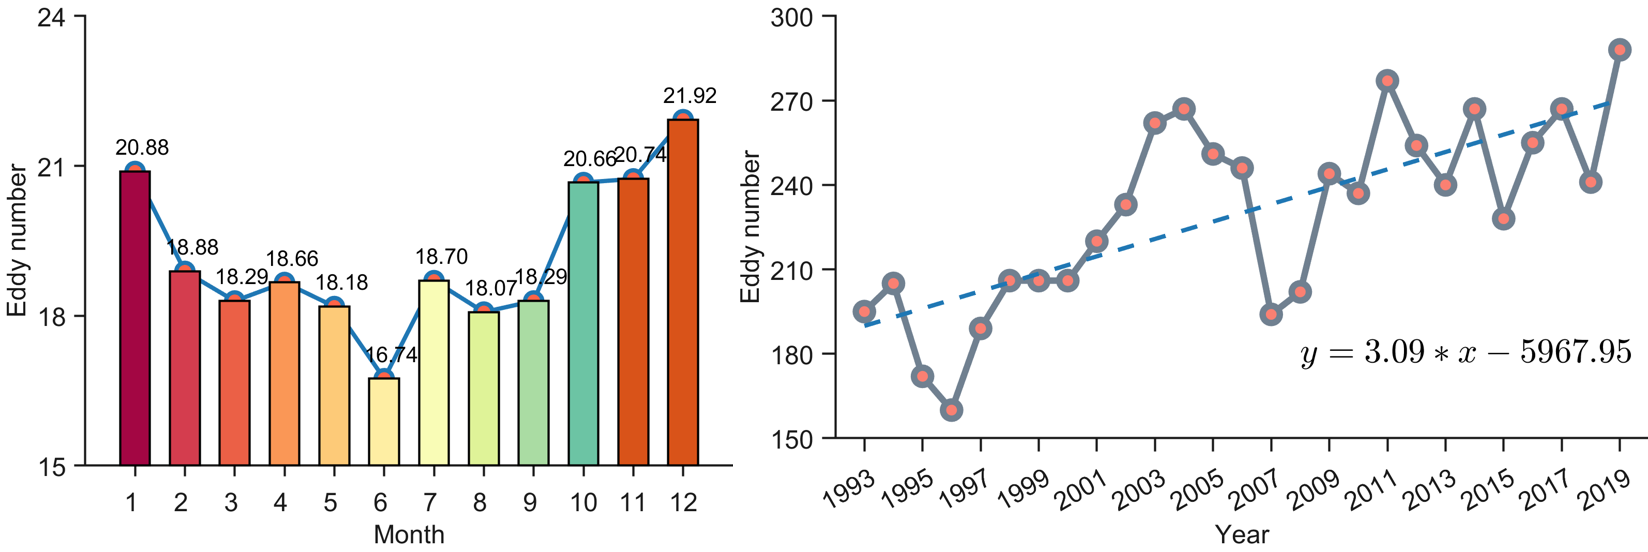
\includegraphics[width = 15cm]{chapter/figure/Eddy number per month and per month.png}
    \caption{Eddy number per month and per month}
    \label{fig:eddy number}
\end{figure}

The average eddy radius is 32.98 km and the standard deviation is 11.31 km. From the eddy radius histogram as shown in section (c) of the figure \ref{Eddy radius map}, we could infer that most of the eddies fall within the range of 20-30 km. The frequency of eddy radius decreases exponentially with increasing radius. From section (b) of the figure \ref{Eddy radius map}, eddy radius does not show an upward or downward trend year by year. Eddies that were generated in 2019 show an average maximum value of 34.41 km while eddies reached the minimum value (31.3 and 31.5 km) in 1996 and 1997. The monthly change of eddy radius shows a minimum value in July and August and a maximum value in December.

Combining the information on eddy number and eddy radius, we may come to the conclusion that in winter, the number and radius of eddies will be reduced due to insufficient energy in the upper ocean.

\begin{figure}
    \centering
    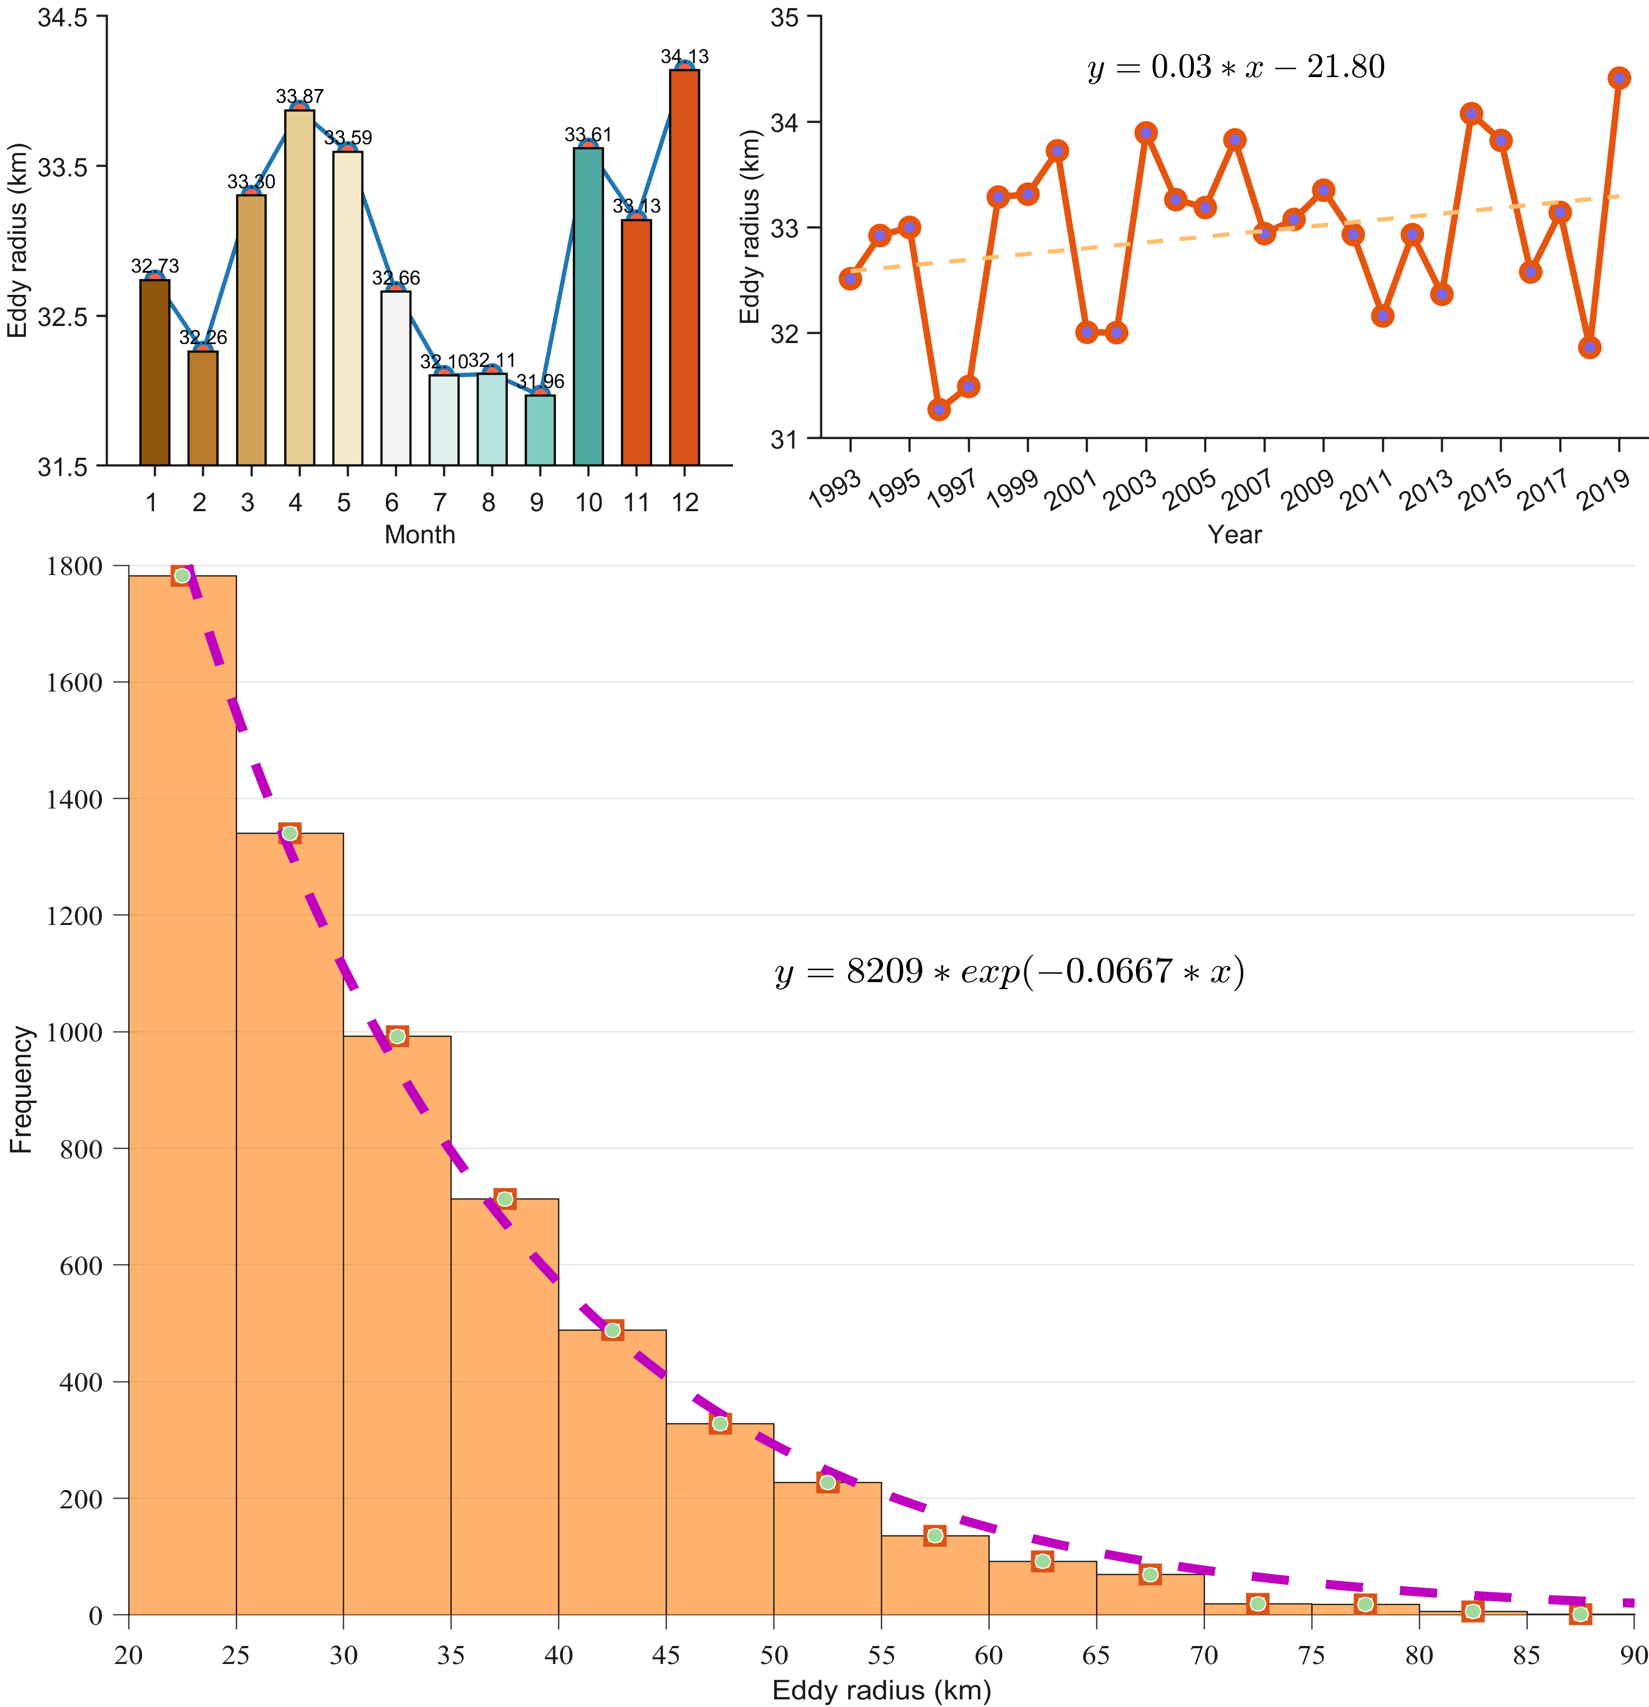
\includegraphics[width =15cm]{chapter/figure/eddy radius2.png}
    \caption{Eddy radius frequency distribution histogram}
    \label{Eddy radius map}
\end{figure}

The figure \ref{radius vs latitude} shows how eddy's radius changes with latitude. From the figure, we could learn that eddies in high latitudes would tend to have a smaller radius, and eddies in lower latitudes would have a larger radius. We also calculated the stretching ratio between the initial eddy area and the final eddy area and the result is shown in figure \ref{enlargement vs latitude}. We infer that eddy would have an inclination to be compressed during the coherent period and the ratio reduces to 0.85 from  $-55^\circ$ S to $-60^\circ $ S, which suggests that the LAVD method may not be so robust in high latitude.

\begin{figure}
    \centering
    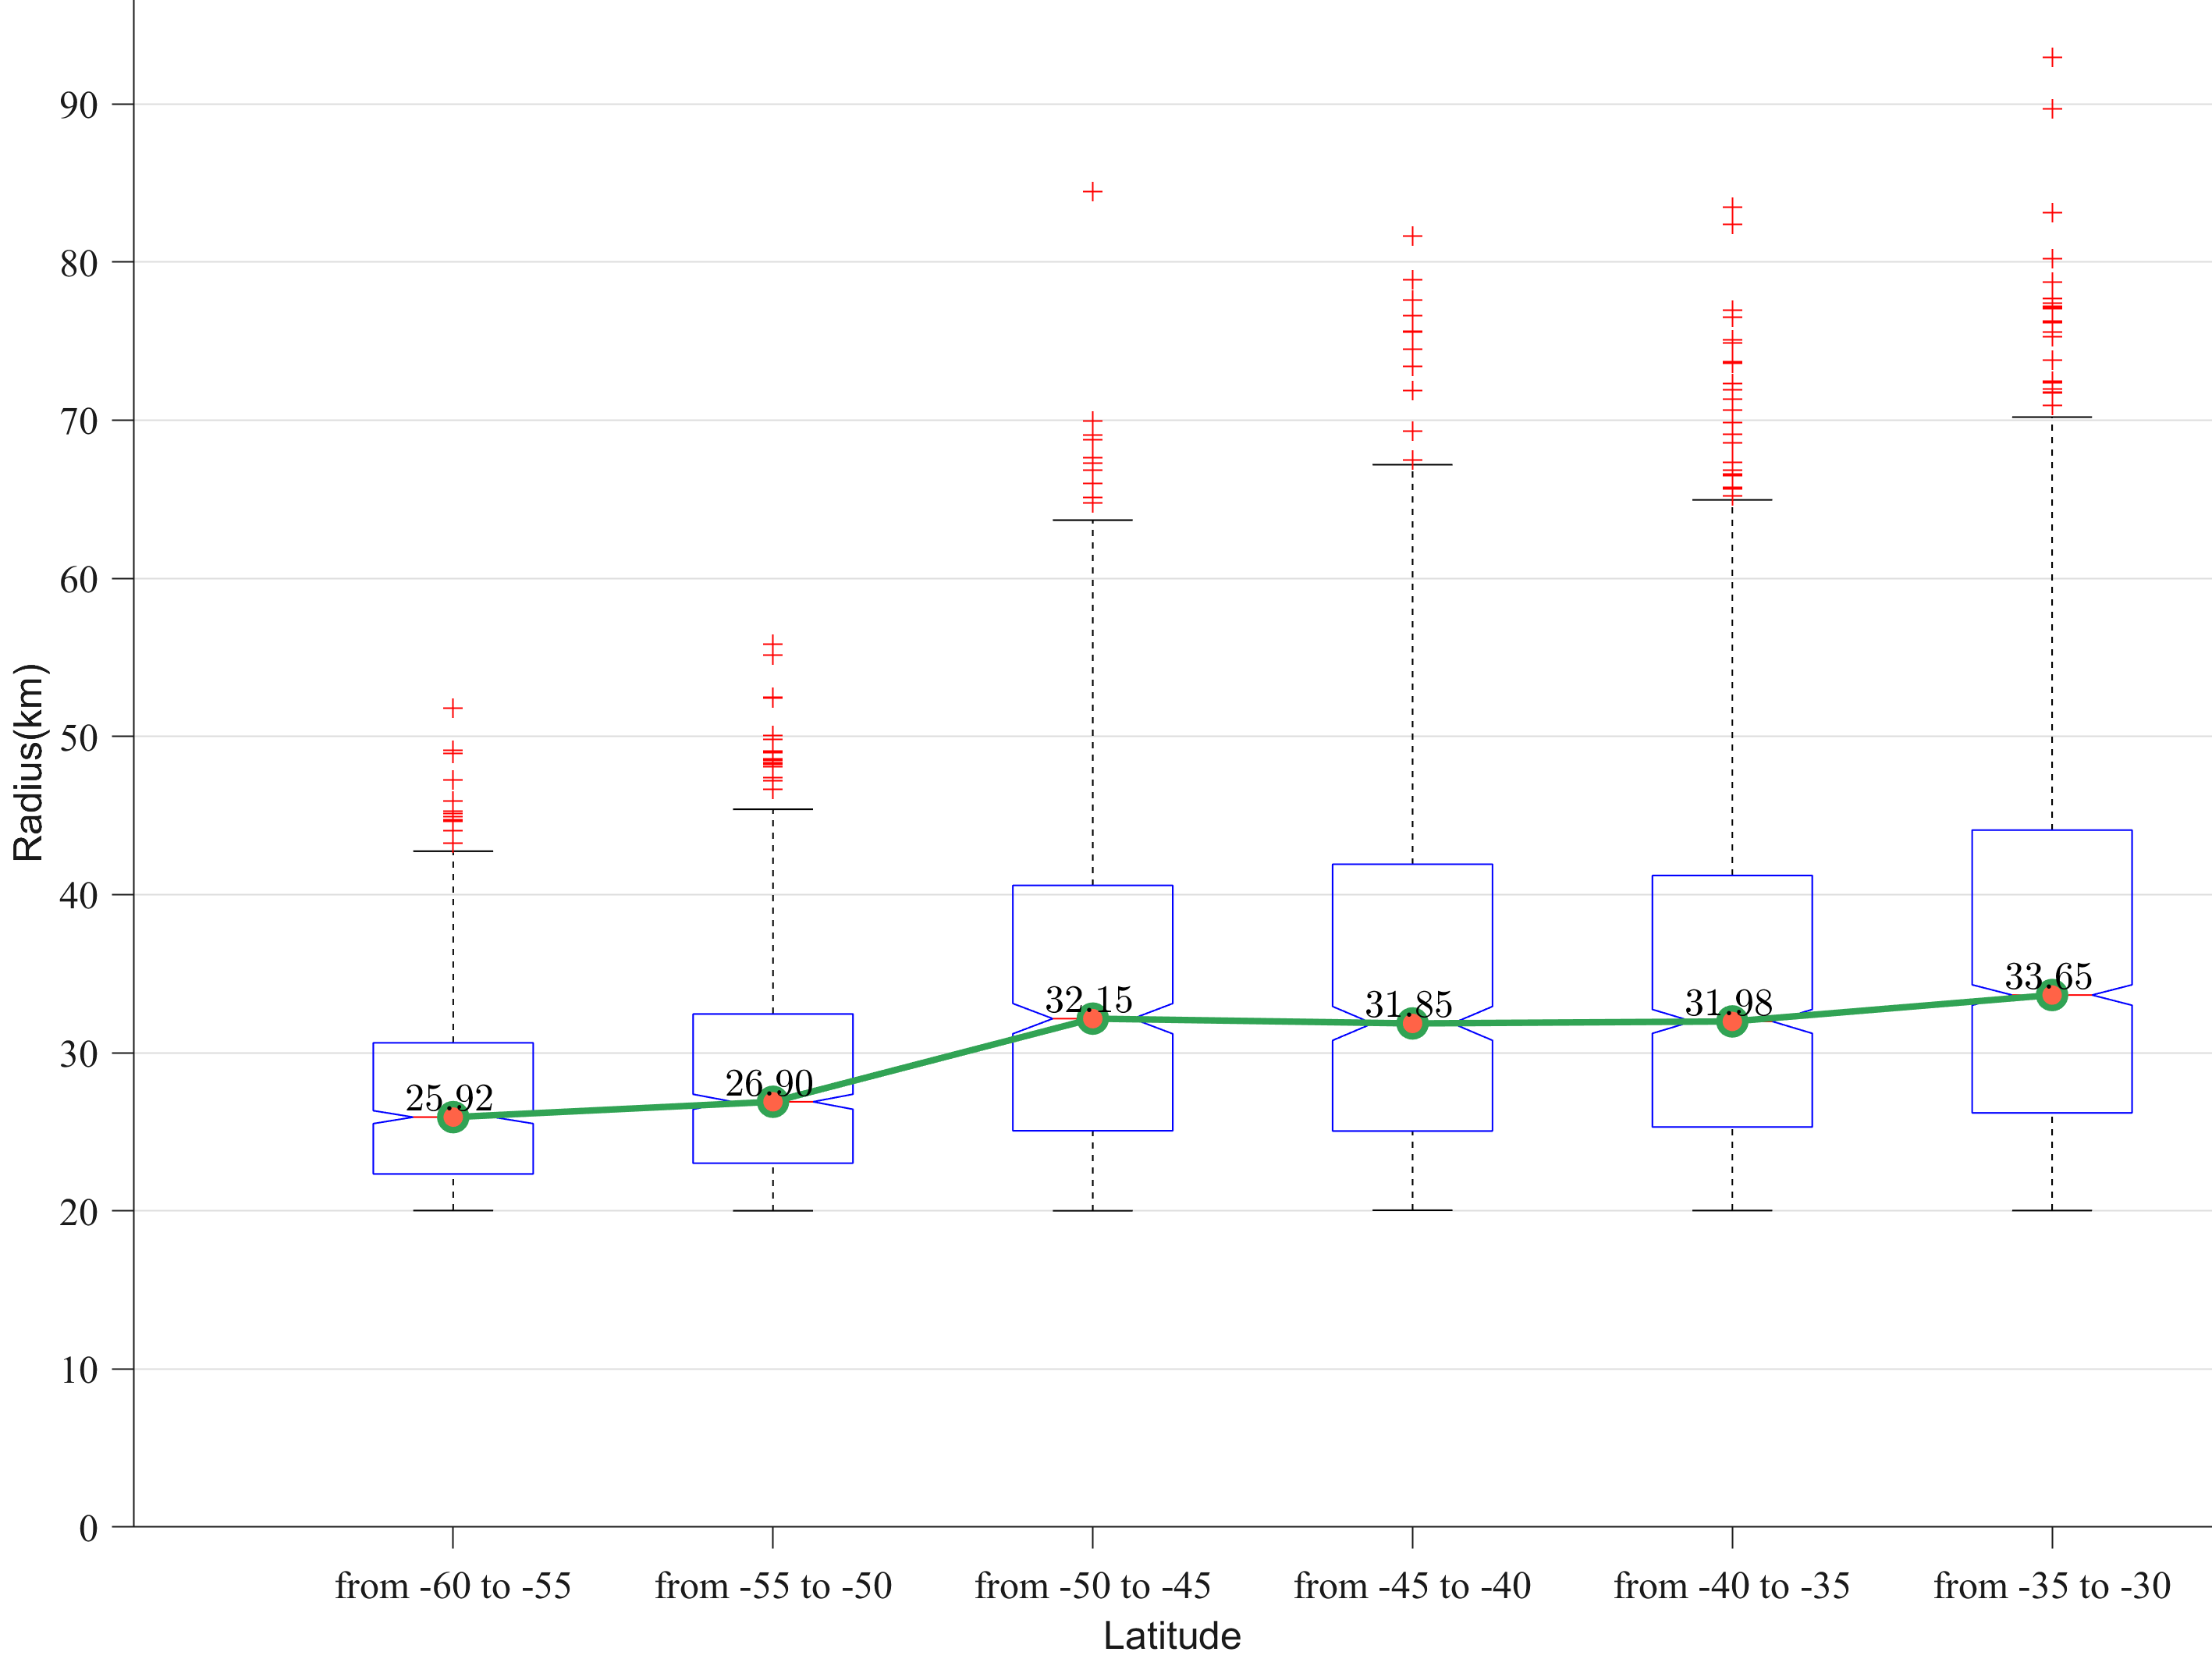
\includegraphics[width = 15cm]{chapter/figure/radius vs latitude.png}
    \caption{Relationship of vortex radius with latitude}
    \label{radius vs latitude}
\end{figure}

\begin{figure}
    \centering
    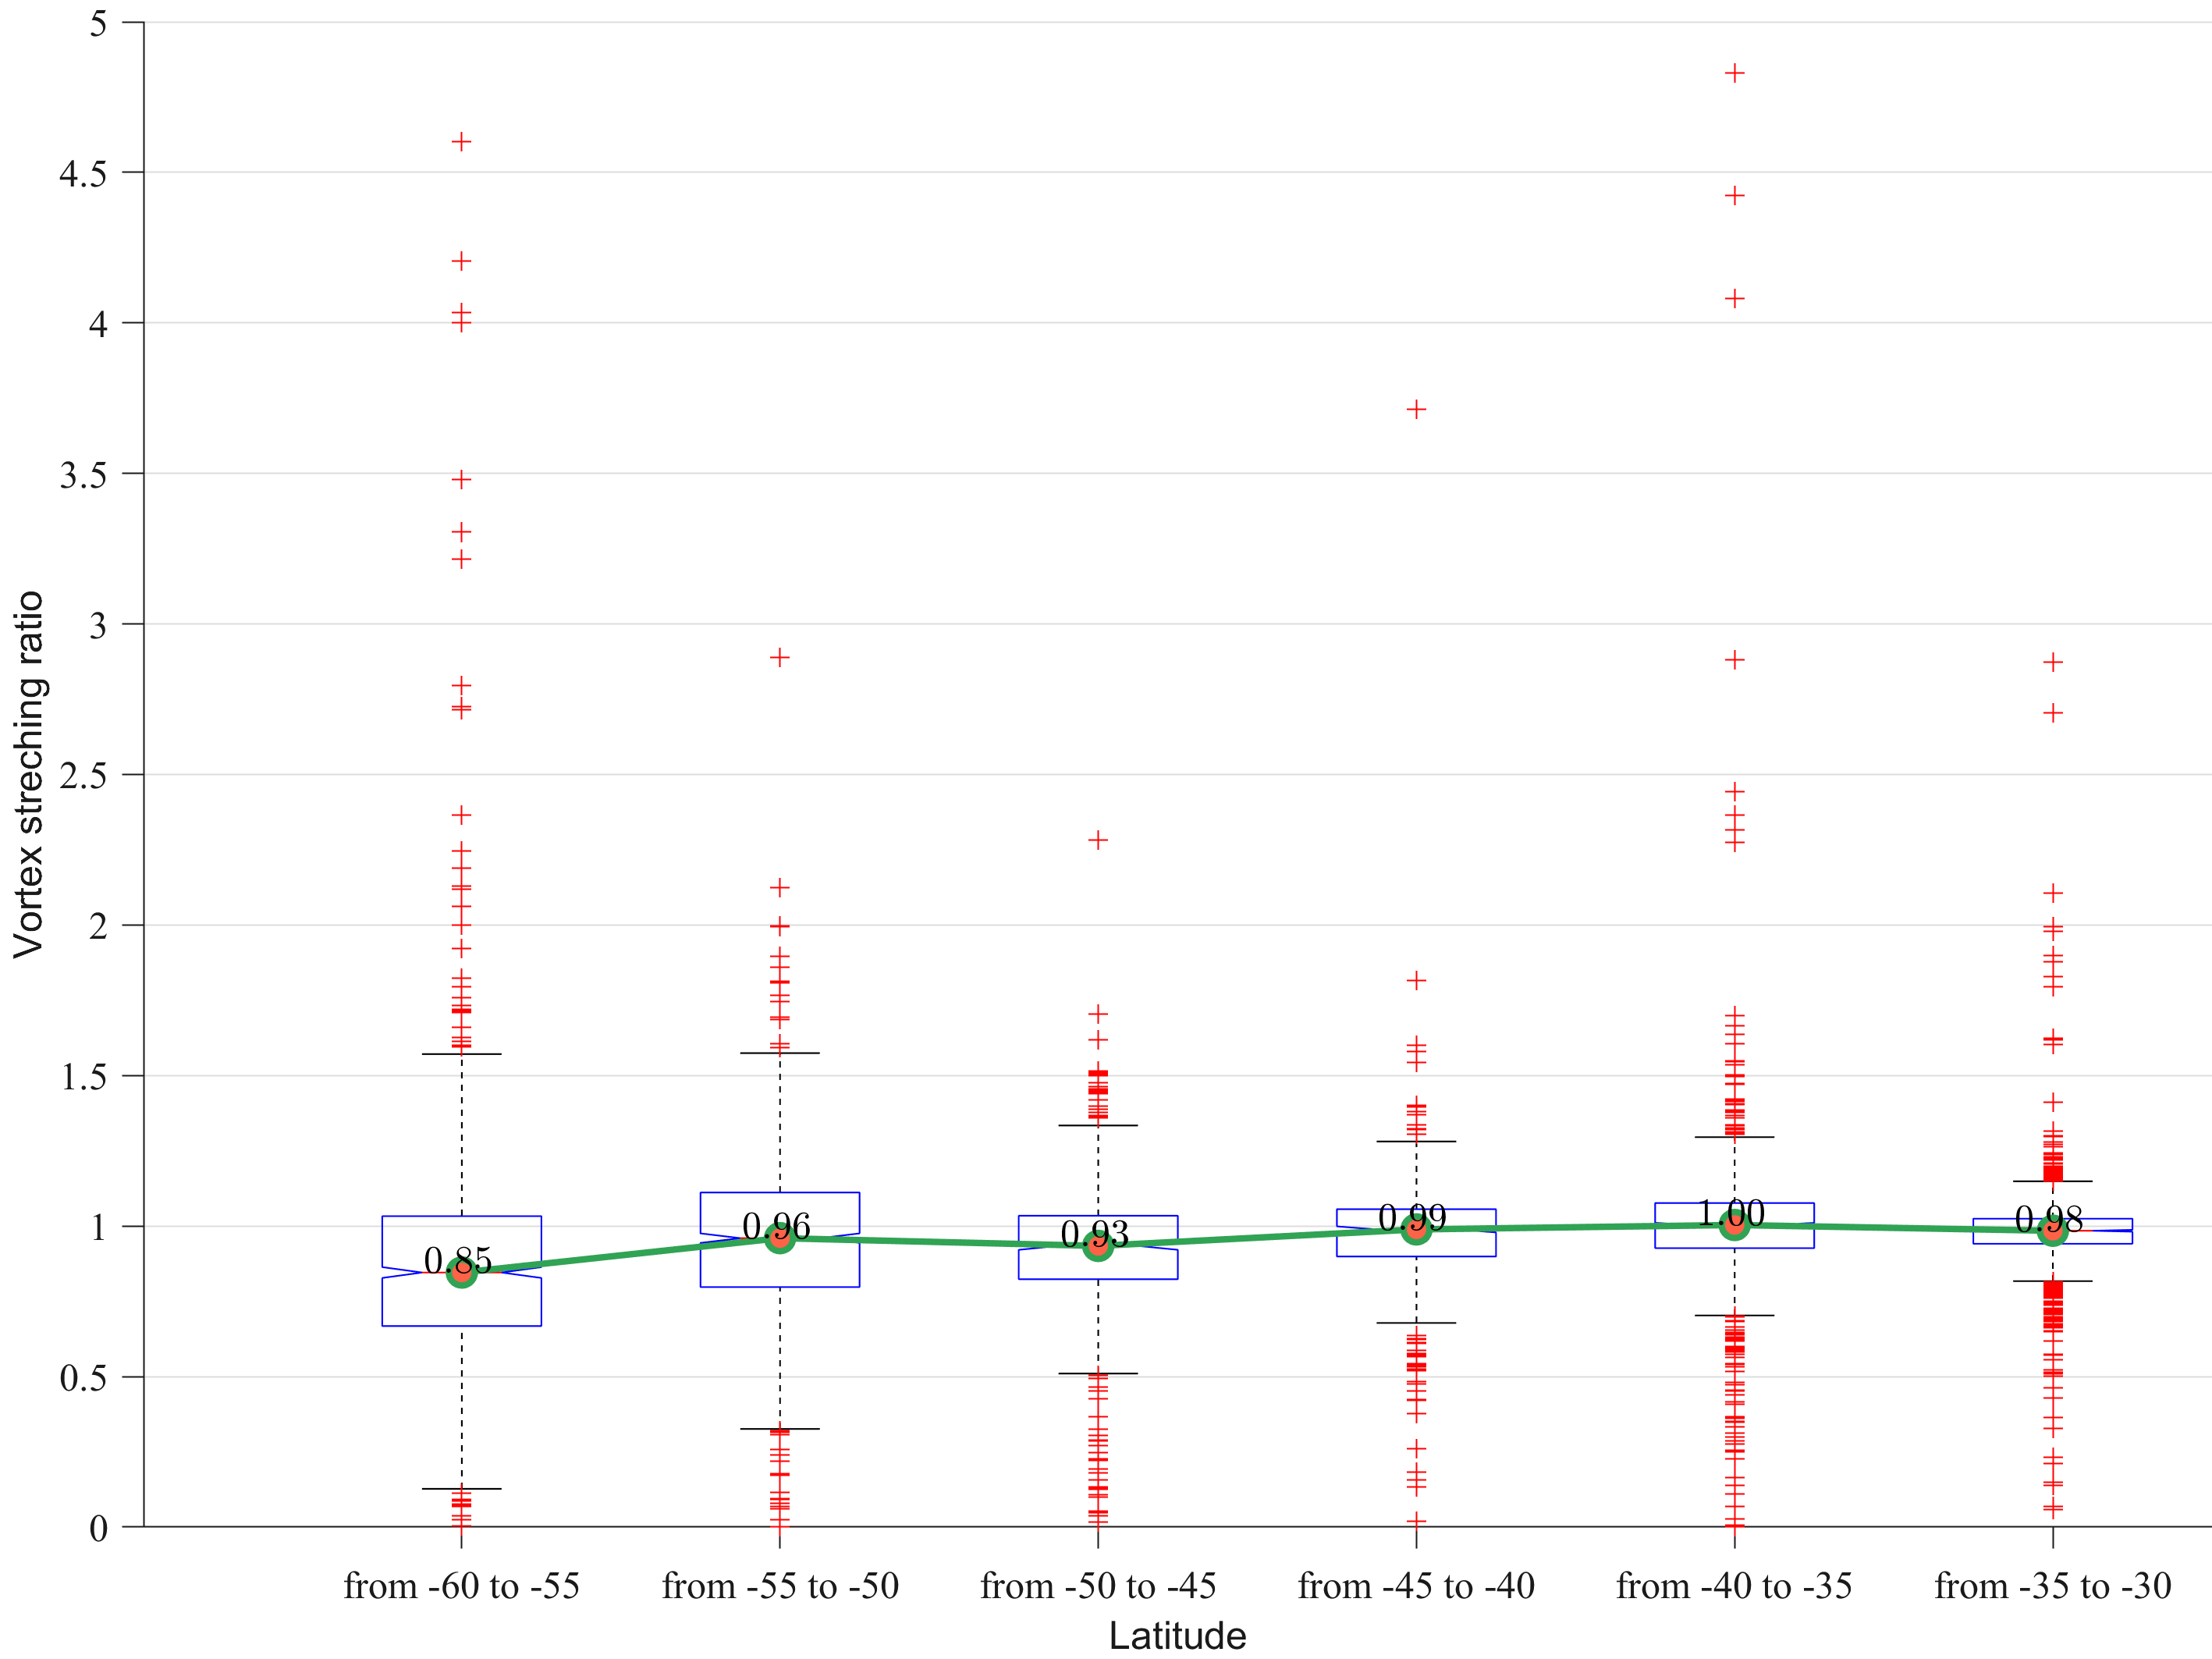
\includegraphics[width = 15cm]{chapter/figure/enlargement vs latitude.png}
    \caption{Relationship of vortex stretching ratio with latitude}
    \label{enlargement vs latitude}
\end{figure}

The figure \ref{velocity vs latitude} demonstrates how eddy propagates in the coherent period. The average propagation speed of the eddy is approximately 5km/day and eddies have the largest propagation speed (about 6.5 km/day) in the middle latitude ranging from $-50^\circ$ S to $-40^\circ$ S. However, the propagation speed will reduce to about 3.6 km/day in higher or lower latitude. There are many outliers for the vortex transport speed in the figure \ref{velocity vs latitude}, which implies the nonlinear effects and causes the vortex moves disorderly. What is more, in most of the cases, the eddy's zonal transport velocity outweighs its meridional component. As shown in figure \ref{Relationship of zonal and meridional velocity with latitude}, the maximum value of zonal velocity is 5.61 km/day near -45°S latitude while the maximum value of meridional velocity is 4.88 km/day at latitudes between -47°S and -50°S. They both show the trend of maximum at intermediate latitudes and decreasing at both low and high latitudes.


\begin{figure}
    \centering
    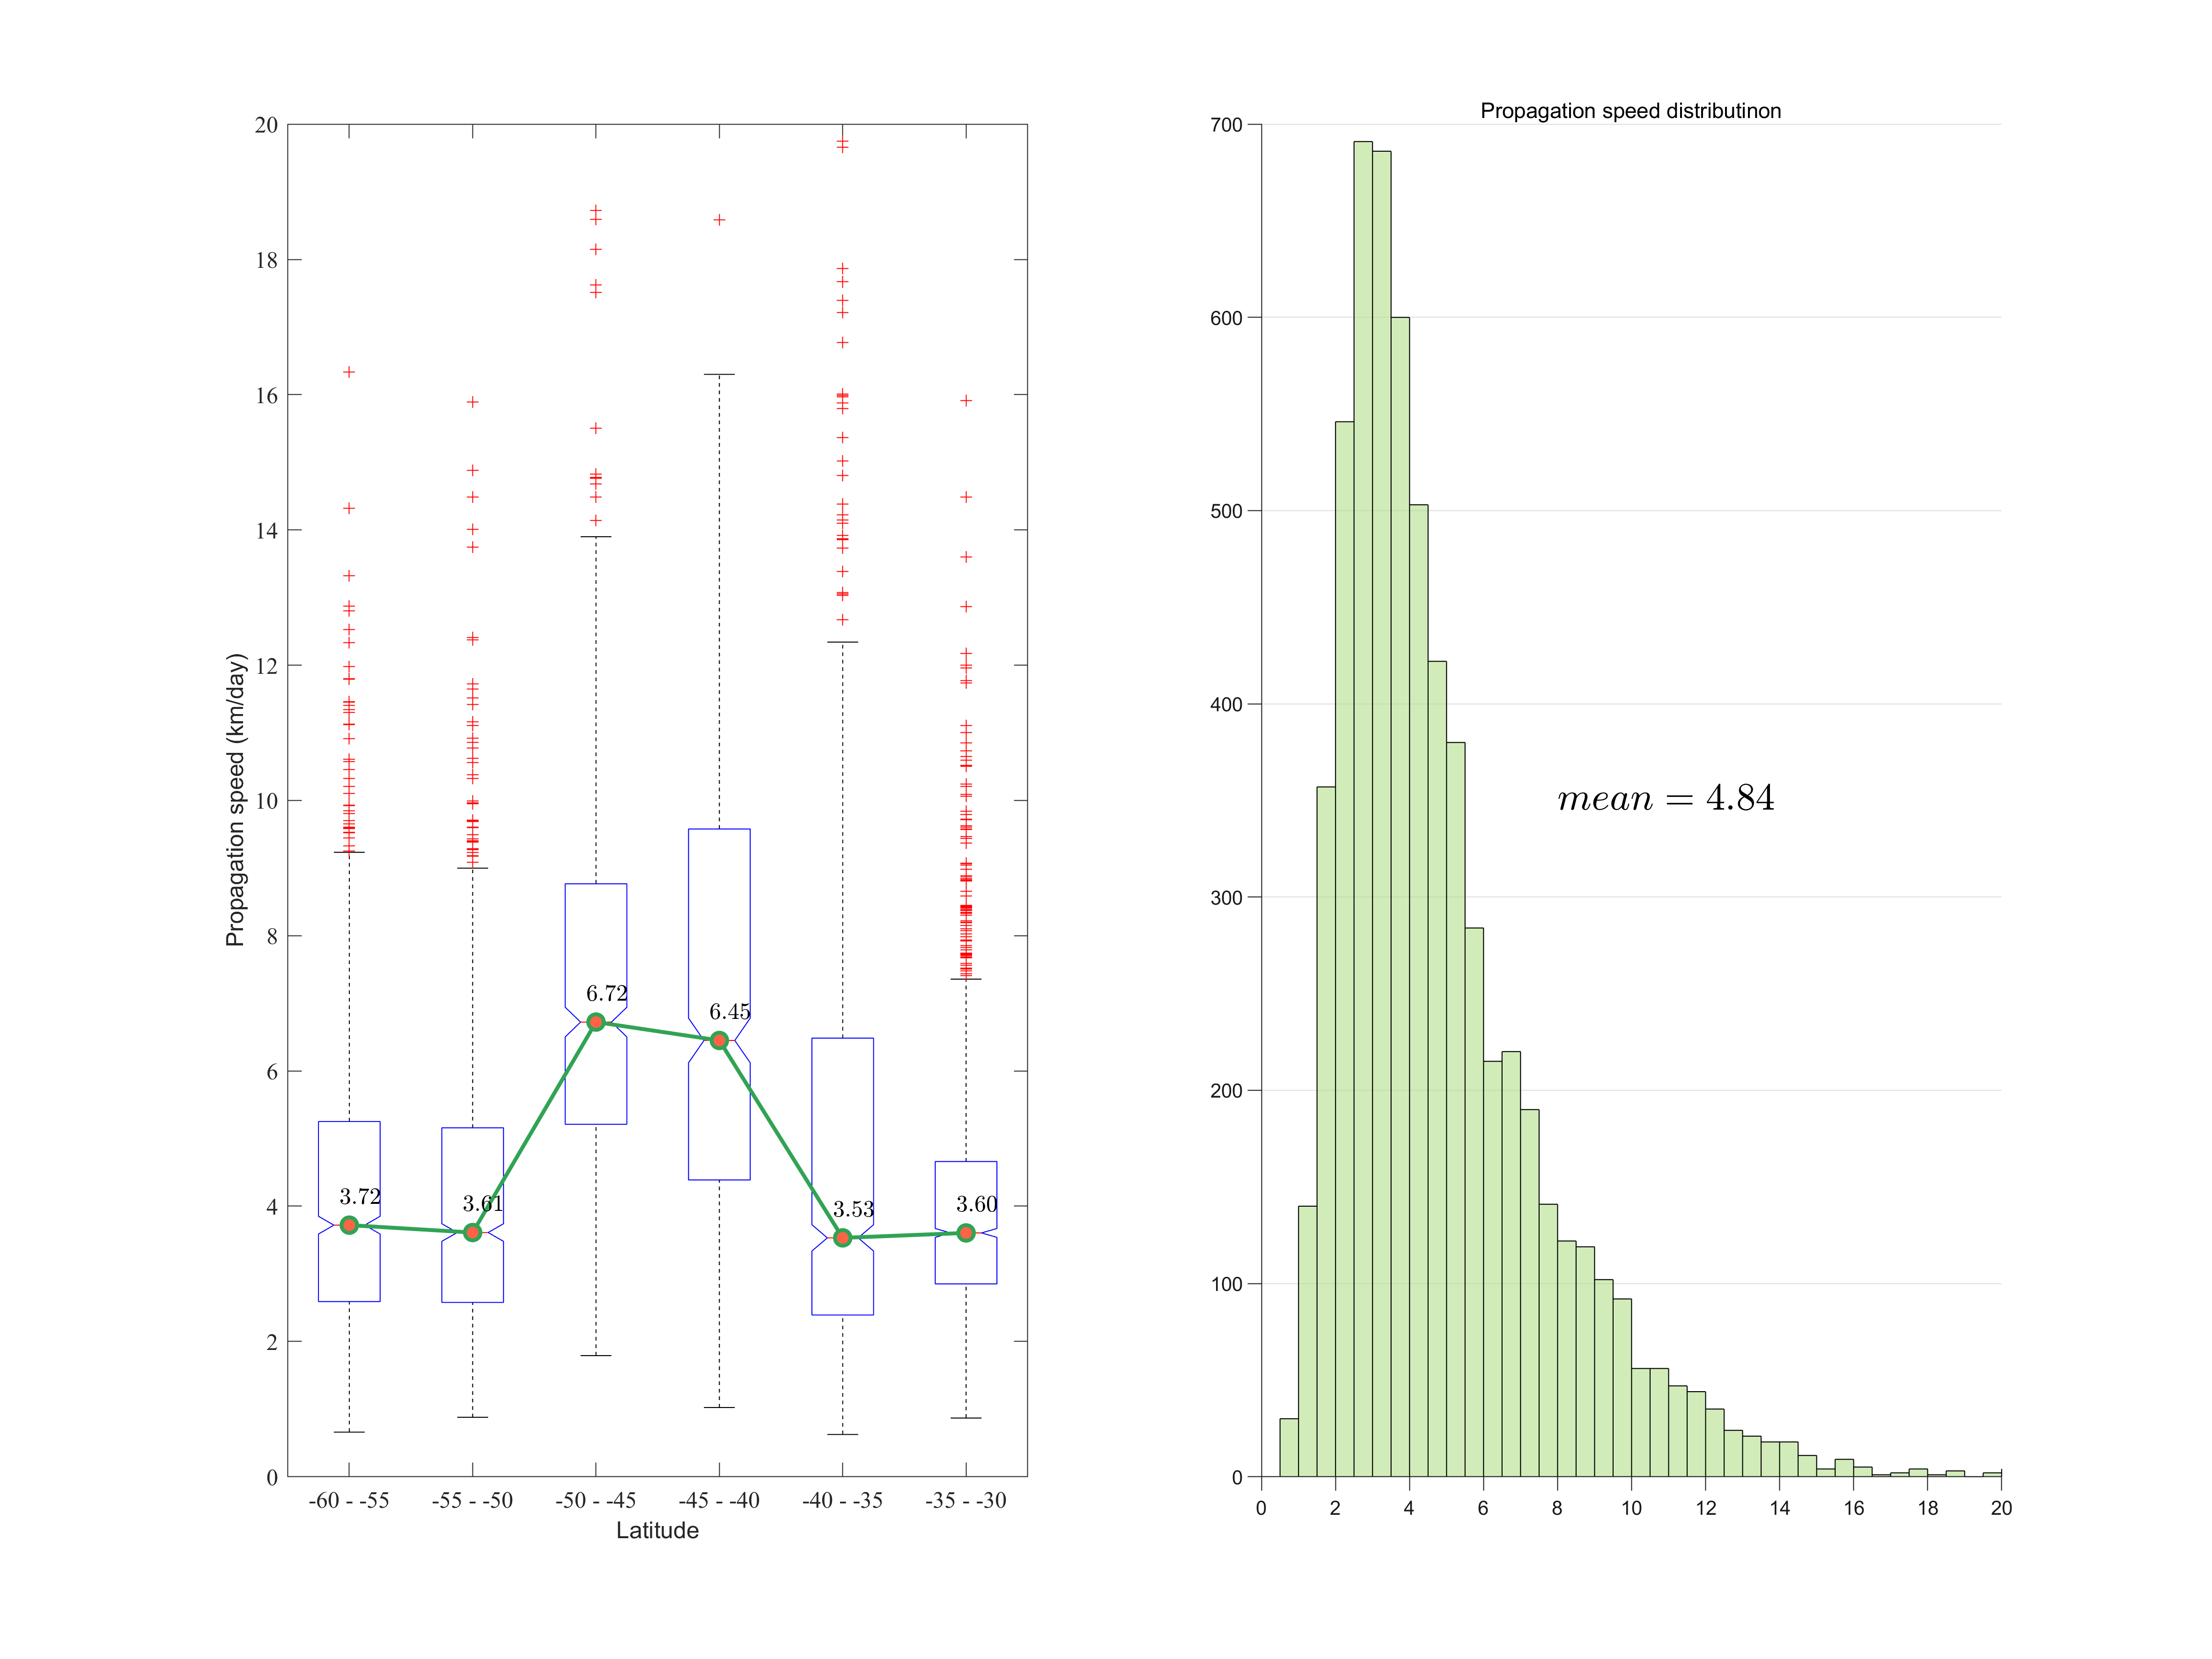
\includegraphics[width = 1.0\textwidth]{chapter/figure/velocity vs latitude.png}
    \caption{Relationship of eddy velocity (km) with latitude}
    \label{velocity vs latitude}
\end{figure}

\begin{figure}
    \centering
    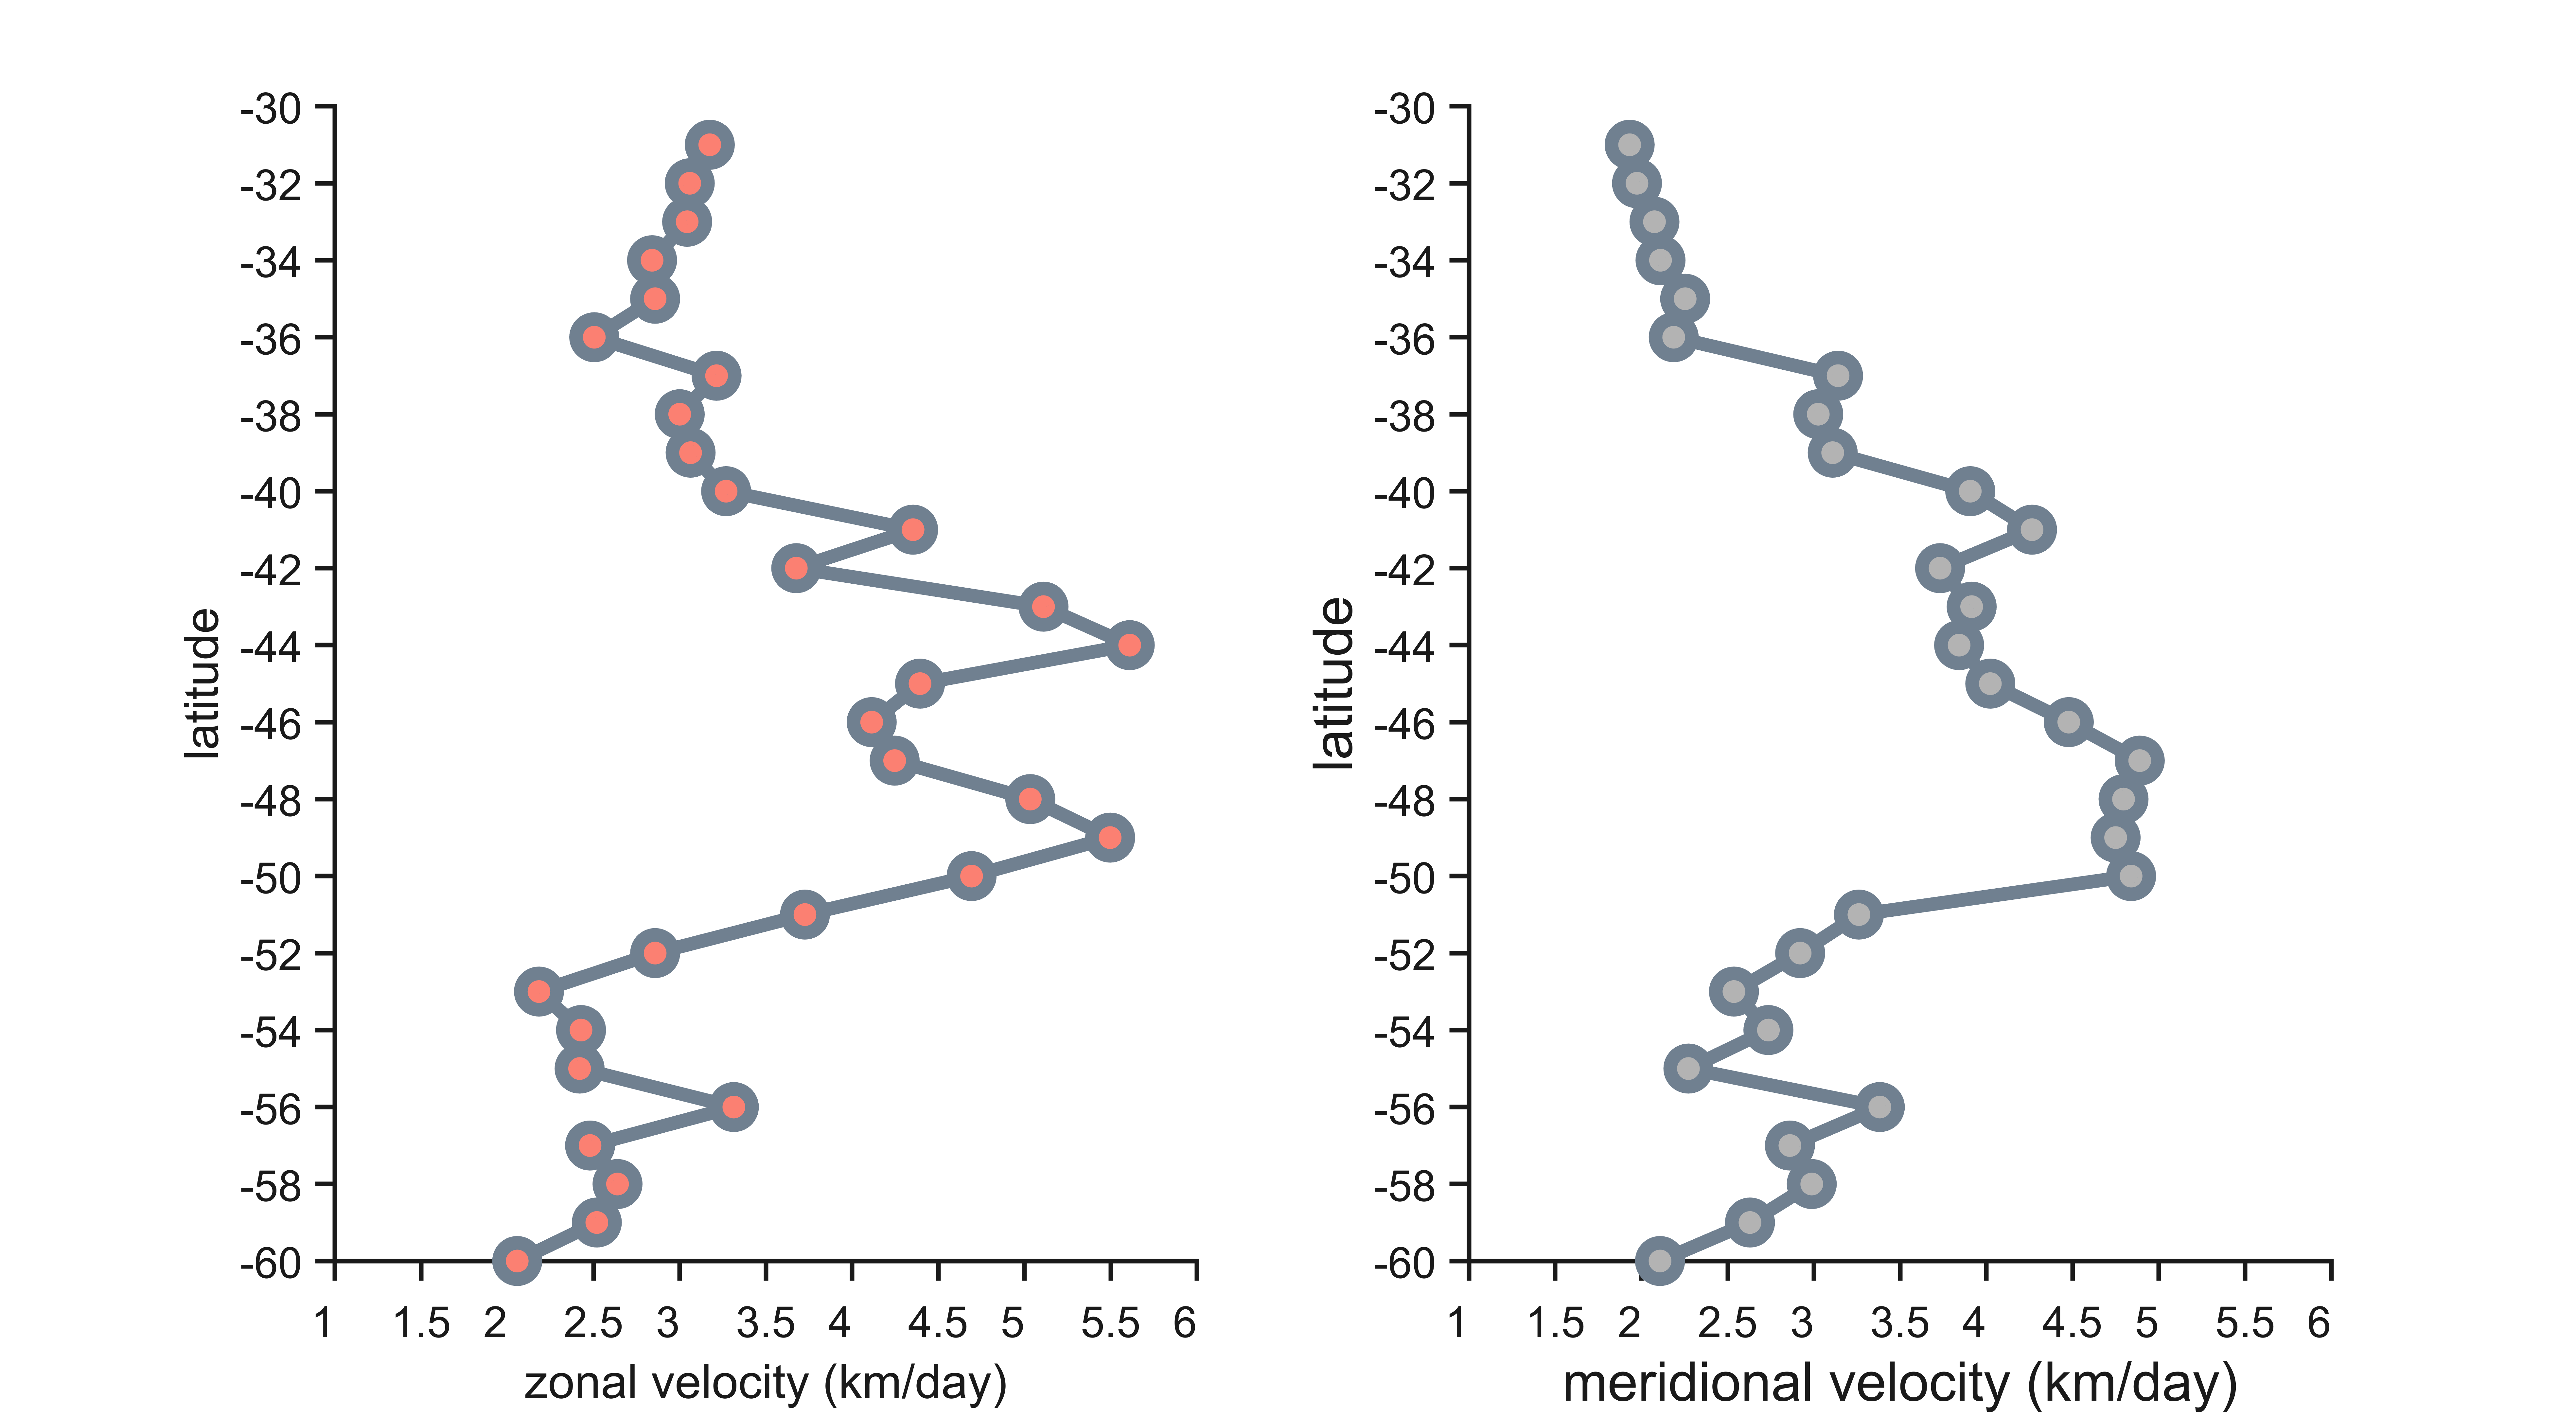
\includegraphics[width = 15cm]{chapter/figure/eddy velocity vs latitude.png}
    \caption{Relationship of zonal and meridional velocity with latitude}
    \label{Relationship of zonal and meridional velocity with latitude}
\end{figure}

The geographical distribution of eddies from 1993 to 2019 is given in the figure \ref{Eddy polarity map}. Among the 6212 vortices, 3336 of them are cyclonic eddies while 2876 of them are anti-cyclonic, which means that cyclonic vortices outweigh anticyclonic ones by about $15\%$. Along the southwest edge of the Argentine Basin, the majority of eddies were cyclonic eddies. Eddies distribute evenly in the Southern Ocean region, while there are more eddies in the northeast part of the Argentine Basin. There is a vortex "vacuum" zone in the center of the Argentine Basin, with only a few vortices remaining there. In the shallow water areas near South America Continent, we detected more anticyclonic vortices. There are few eddies detected in the coastal region since the deviation of altimeter data near the coastline is rather high due to the influence of tides and coastal waves. In the water regions connecting the Southern Ocean and Argentine Basin, eddies distribute in a striped pattern.

\begin{figure}
    \centering
    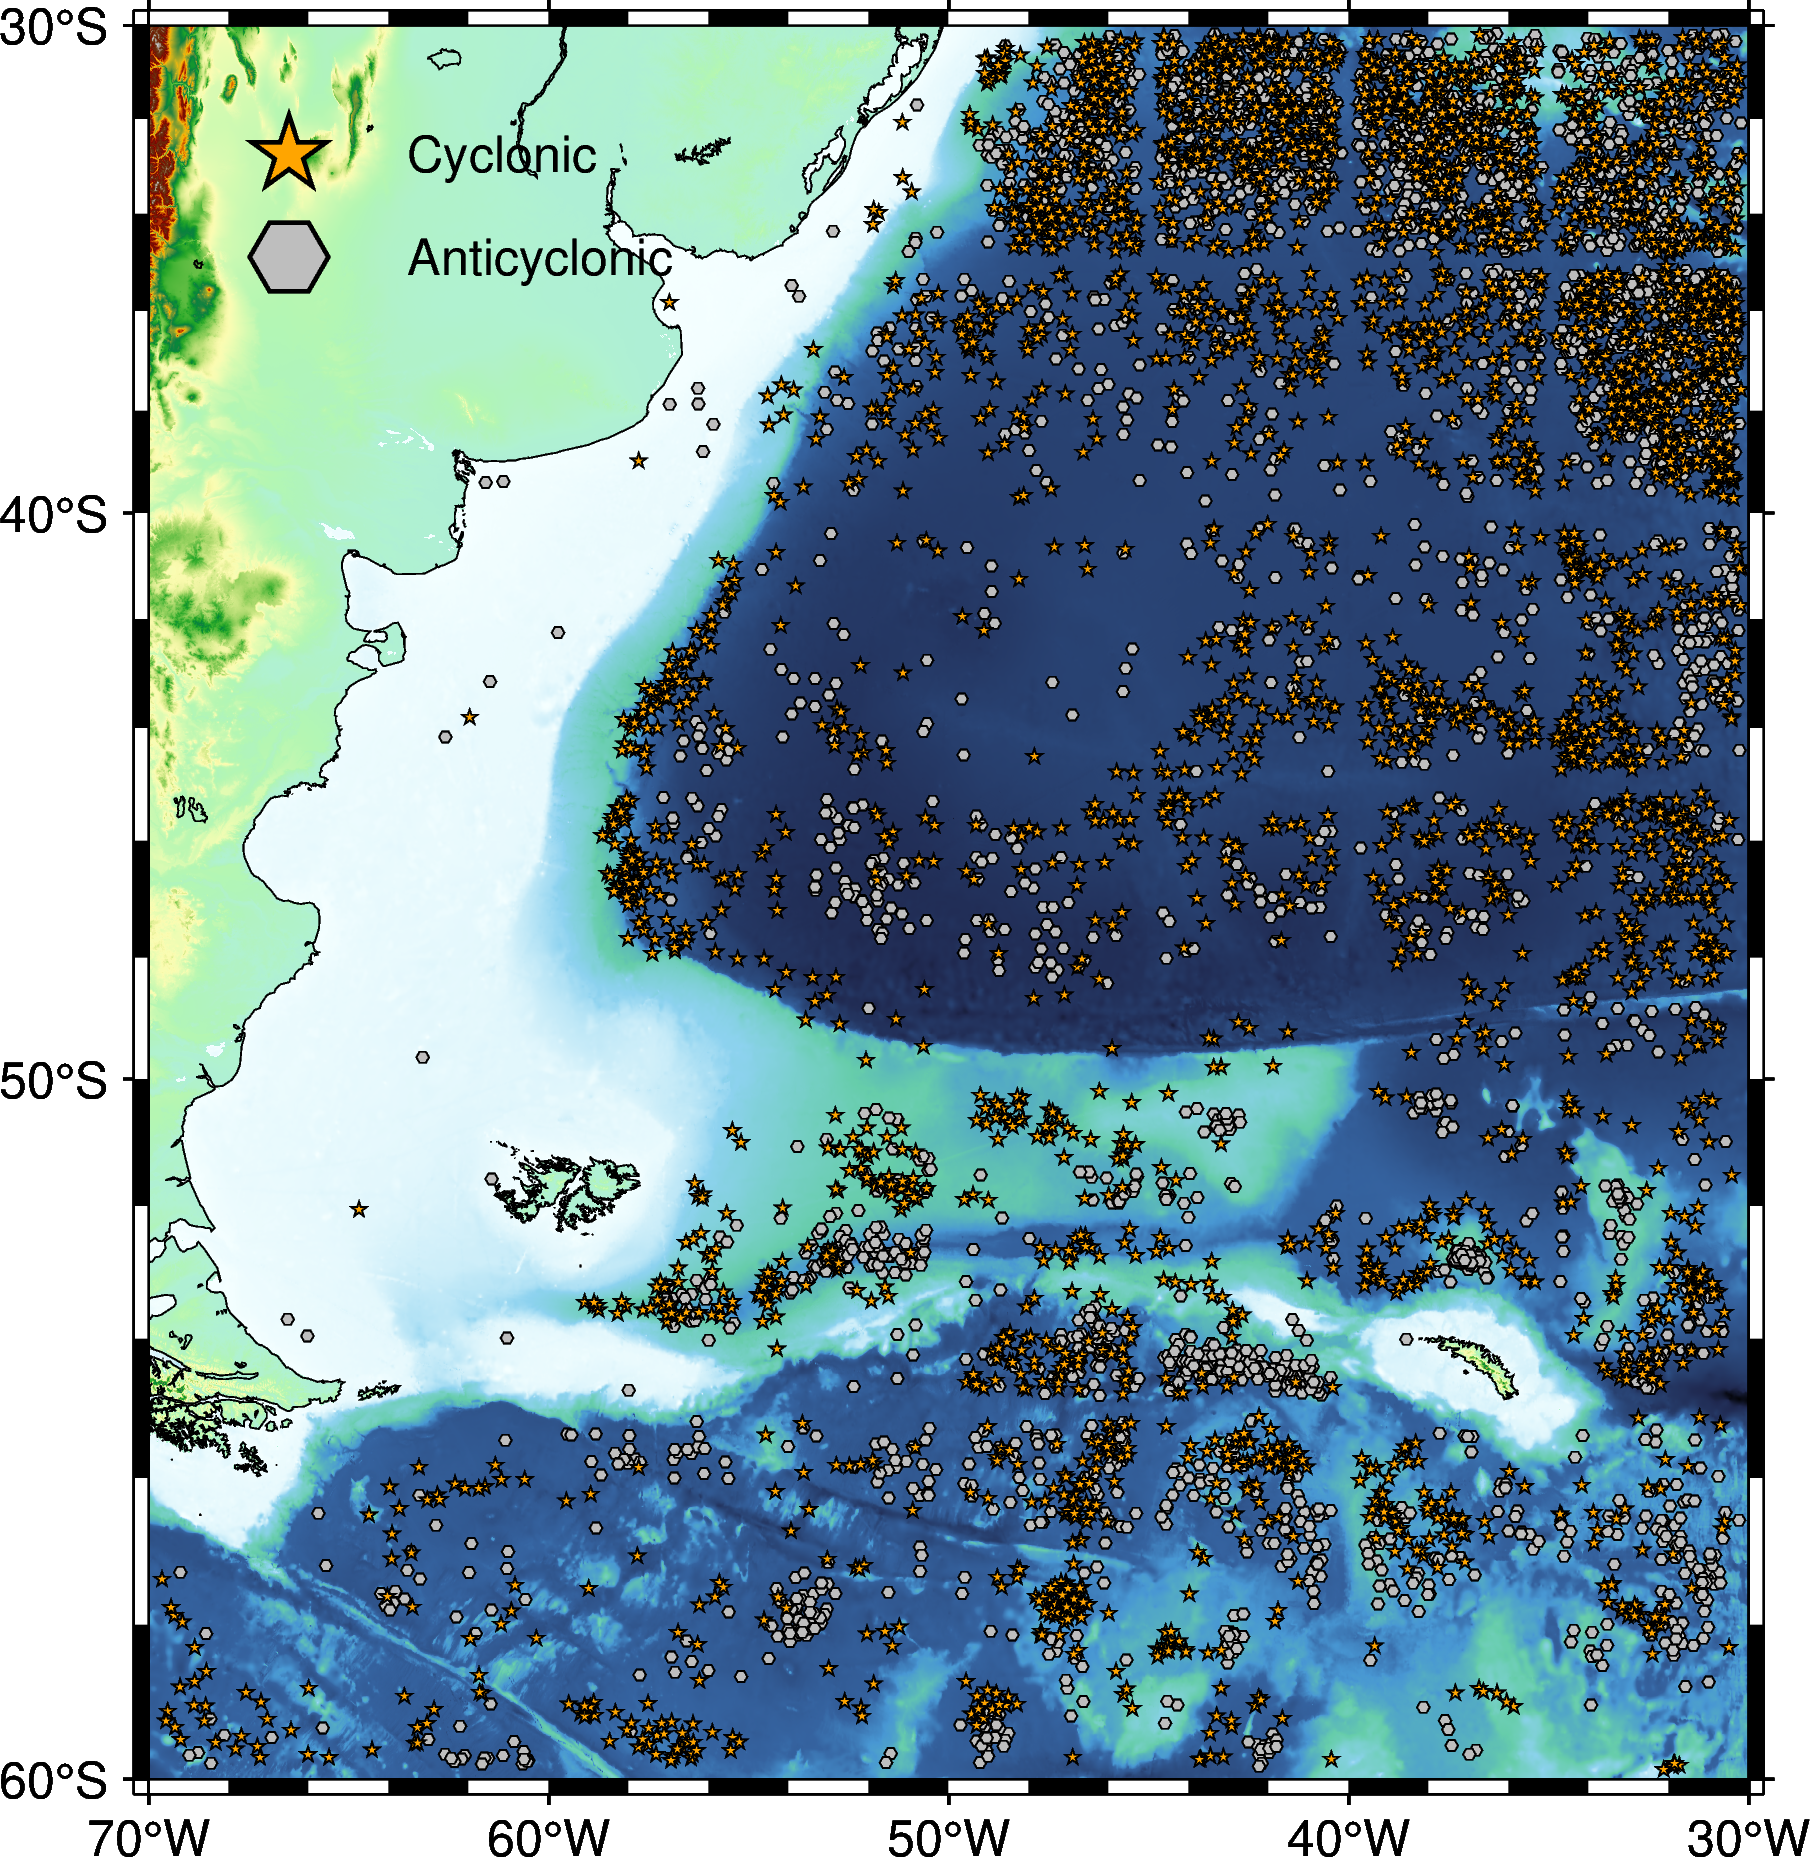
\includegraphics[width = 15cm]{chapter/figure/eddy polarity map.png}
    \caption{Eddy polarity distribution map}
    \label{Eddy polarity map}
\end{figure}

The figure \ref{eddy number vs Polarity} shows annual variation and monthly variation of eddy number and vortex radius of cyclonic and anti-cyclonic eddies. Anti-cyclonic eddies have distinct seasonal variations while seasonal number differences of cyclonic eddies are small. In all months, the number of cyclonic vortices is higher than the anti-cyclonic ones. The average number of anti-cyclonic eddies appearing in June is 7.59, which is the lowest in all months. Anti-cyclonic eddy number reaches the minimum value in winter and it increases slowly and reaches a maximum in winter. Annual variation characteristics of vortex numbers tell us that in most of the years, cyclonic eddy numbers outweigh anti-cyclonic ones while the opposite rule was observed in 1995 and 1996. An average of 124 cyclonic vortices and 107 anti-cyclonic eddies are generated each year. Both the number of cyclonic eddies and anti-cyclonic eddies would increase, and the increasing trend of cyclonic eddies is more obvious. The maximum number of annual cyclonic eddies found in the Argentine Basin is 168 in 2019 while the maximum number of annual anti-cyclonic eddies is 133 in 2006.

\begin{figure}
    \centering
    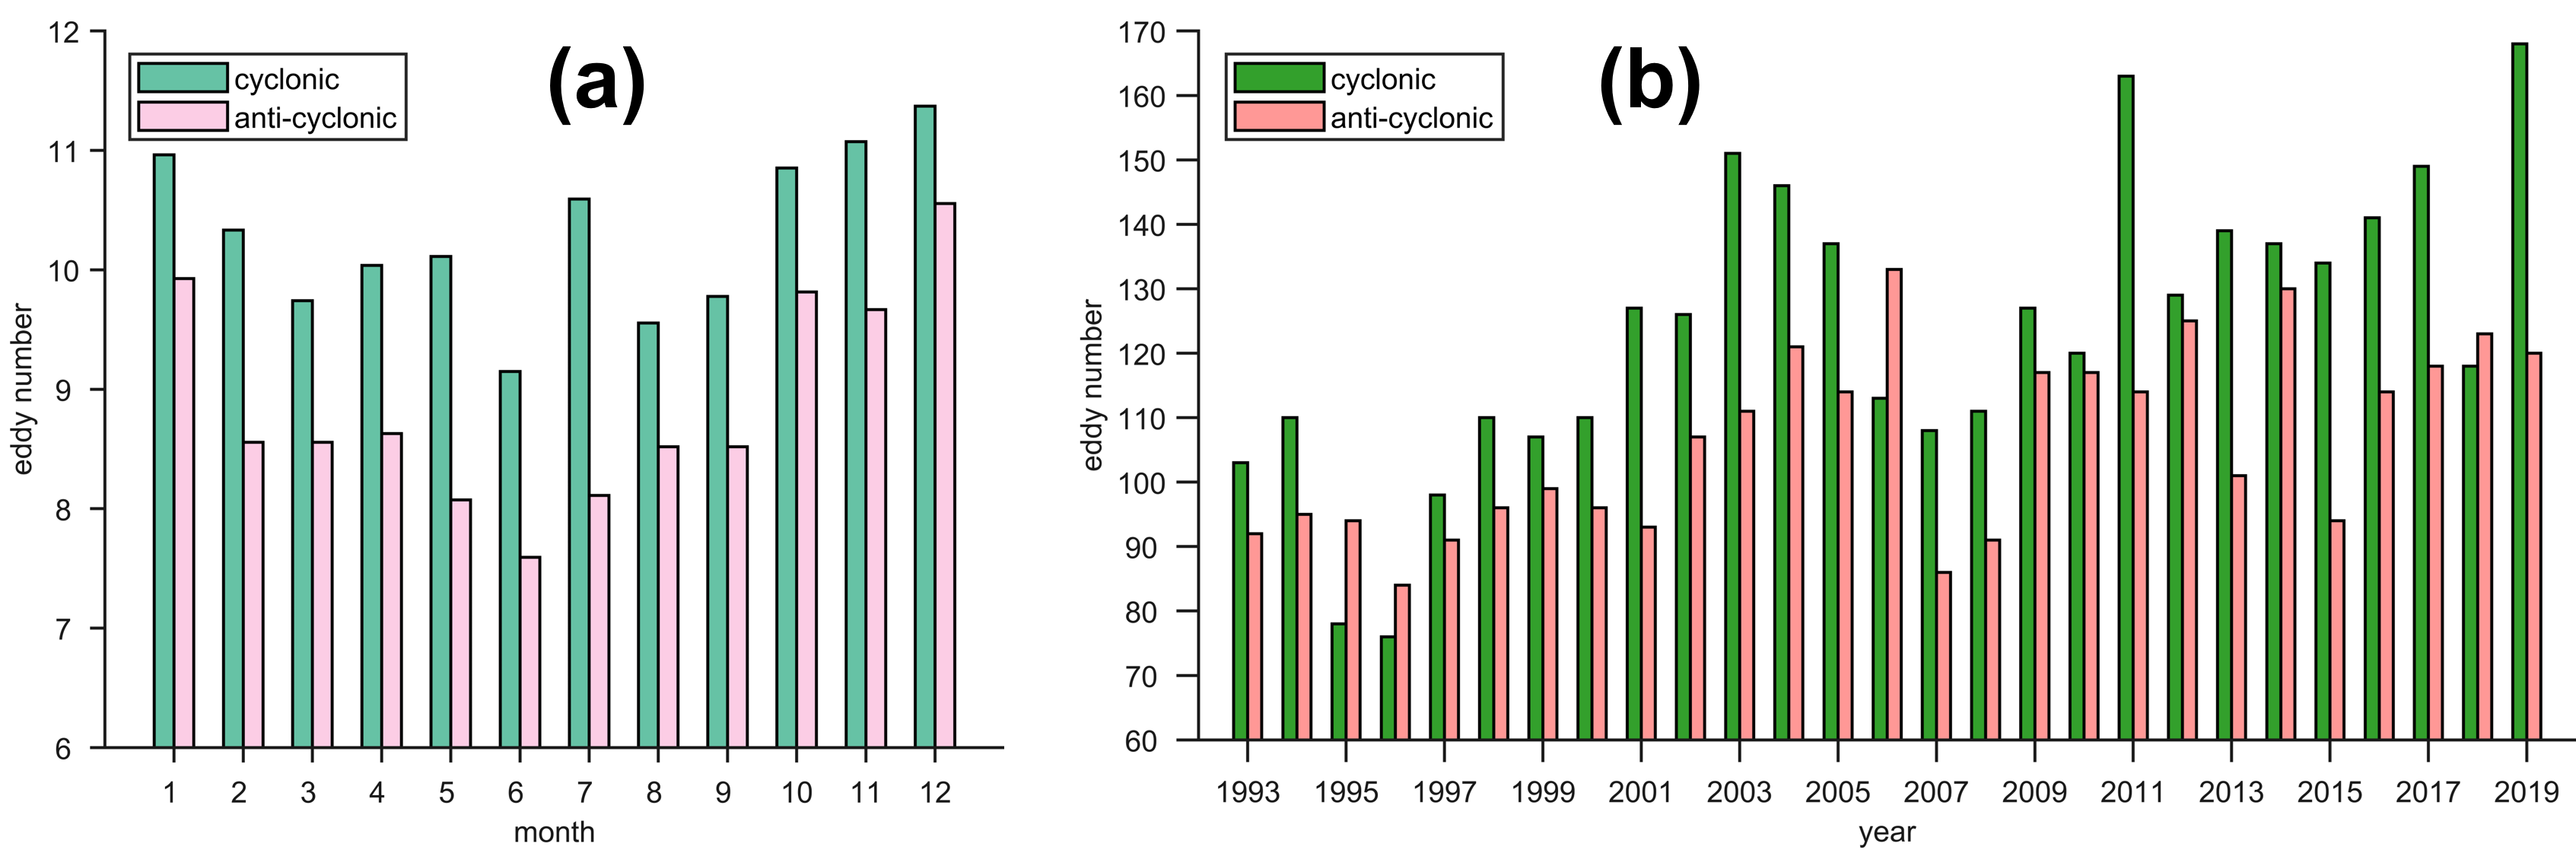
\includegraphics[width = 15cm]{chapter/figure/eddy number vs Polarity.png}
    \caption{Monthly and annual patterns of eddy number of different polarities}
    \label{eddy number vs Polarity}
\end{figure}

Figure \ref{eddy radius vs type} shows how vortex polarity affects vortex size. Before 2010, the diameter of the anticyclonic vortex was more extensive than that of the cyclonic vortex. Since 2007, the radius of cyclonic vortex began to grow and has become bigger than anti-cyclonic ones. From the figure, we could learn that different types of eddies have different seasonal patterns. The average monthly minimum radius of cyclonic eddies is 31.52 km in September while the minimum monthly radius of anti-cyclonic vortices is about 32 km in June. They both show maximum value in December.

\begin{figure}
    \centering
    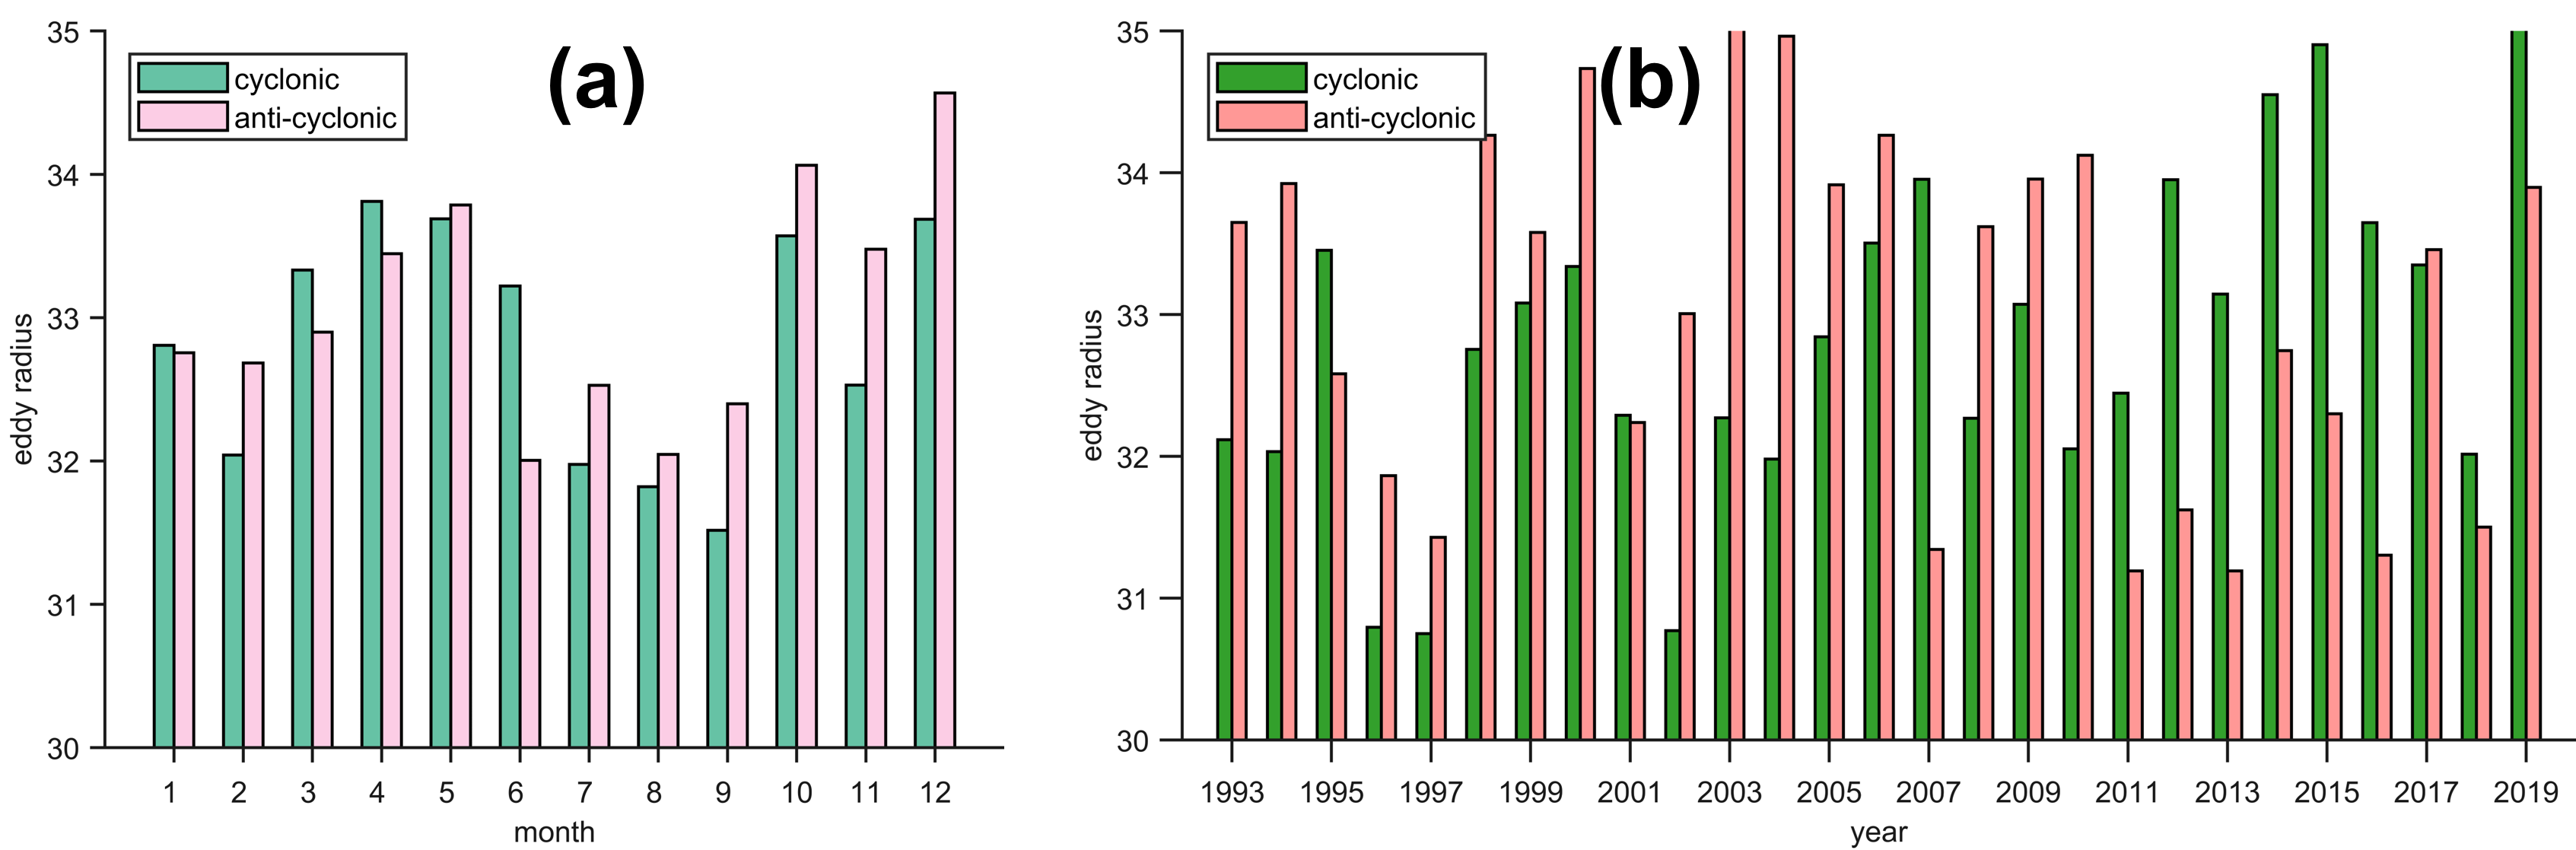
\includegraphics[width = 15cm]{chapter/figure/eddy radius vs type.png}
    \caption{Monthly and annual patterns of eddy radius of different polarities}
    \label{eddy radius vs type}
\end{figure}

In Figure \ref{eddy classification map_SNWE2}, we compared eddies' initial position and final position from 1993 to 2019 and the figure shows the direction of eddy propagation. About $59\%$ of the eddies would travel northward, and only $41\%$ would travel southward. Anticyclonic vortices are more inclined to transport to the poles. In the east-west direction, about $63\%$ of the eddies travel westward, and only $37\%$ of them travel to the east.

From the map, we could learn that even in the northern part of the Argentine Basin which is affected by the southward Brazil Current, most of the eddies would tend to travel northward, which suggests an opposite direction of the mean flow and eddy flow. Along the border connecting the shallow water region and Argentine Basin, we could learn that eddies in the northern part of the border have an inclination to travel southward and eddies in the southern part have a trend to travel northward. This is coincident with the southward Brazil Current and northward Malvinas Current. In the middle of the Argentine Basin, eddies' travel pattern agrees with the Zapiola Anticyclone.

In the Southern Ocean region, most of the observed eddies travel eastward because of the Antarctic Circumpolar Current. On the northern part of the Argentine Basin, the majority of the eddies propagate westward.
In the center of the basin, because of the Argentine Gyre and branch of the Brazil Current, we could see that at the southern edge of the basin, eddies would tend to move eastward while eddies would move to the west in the middle of the basin.

\begin{figure}
    \centering
    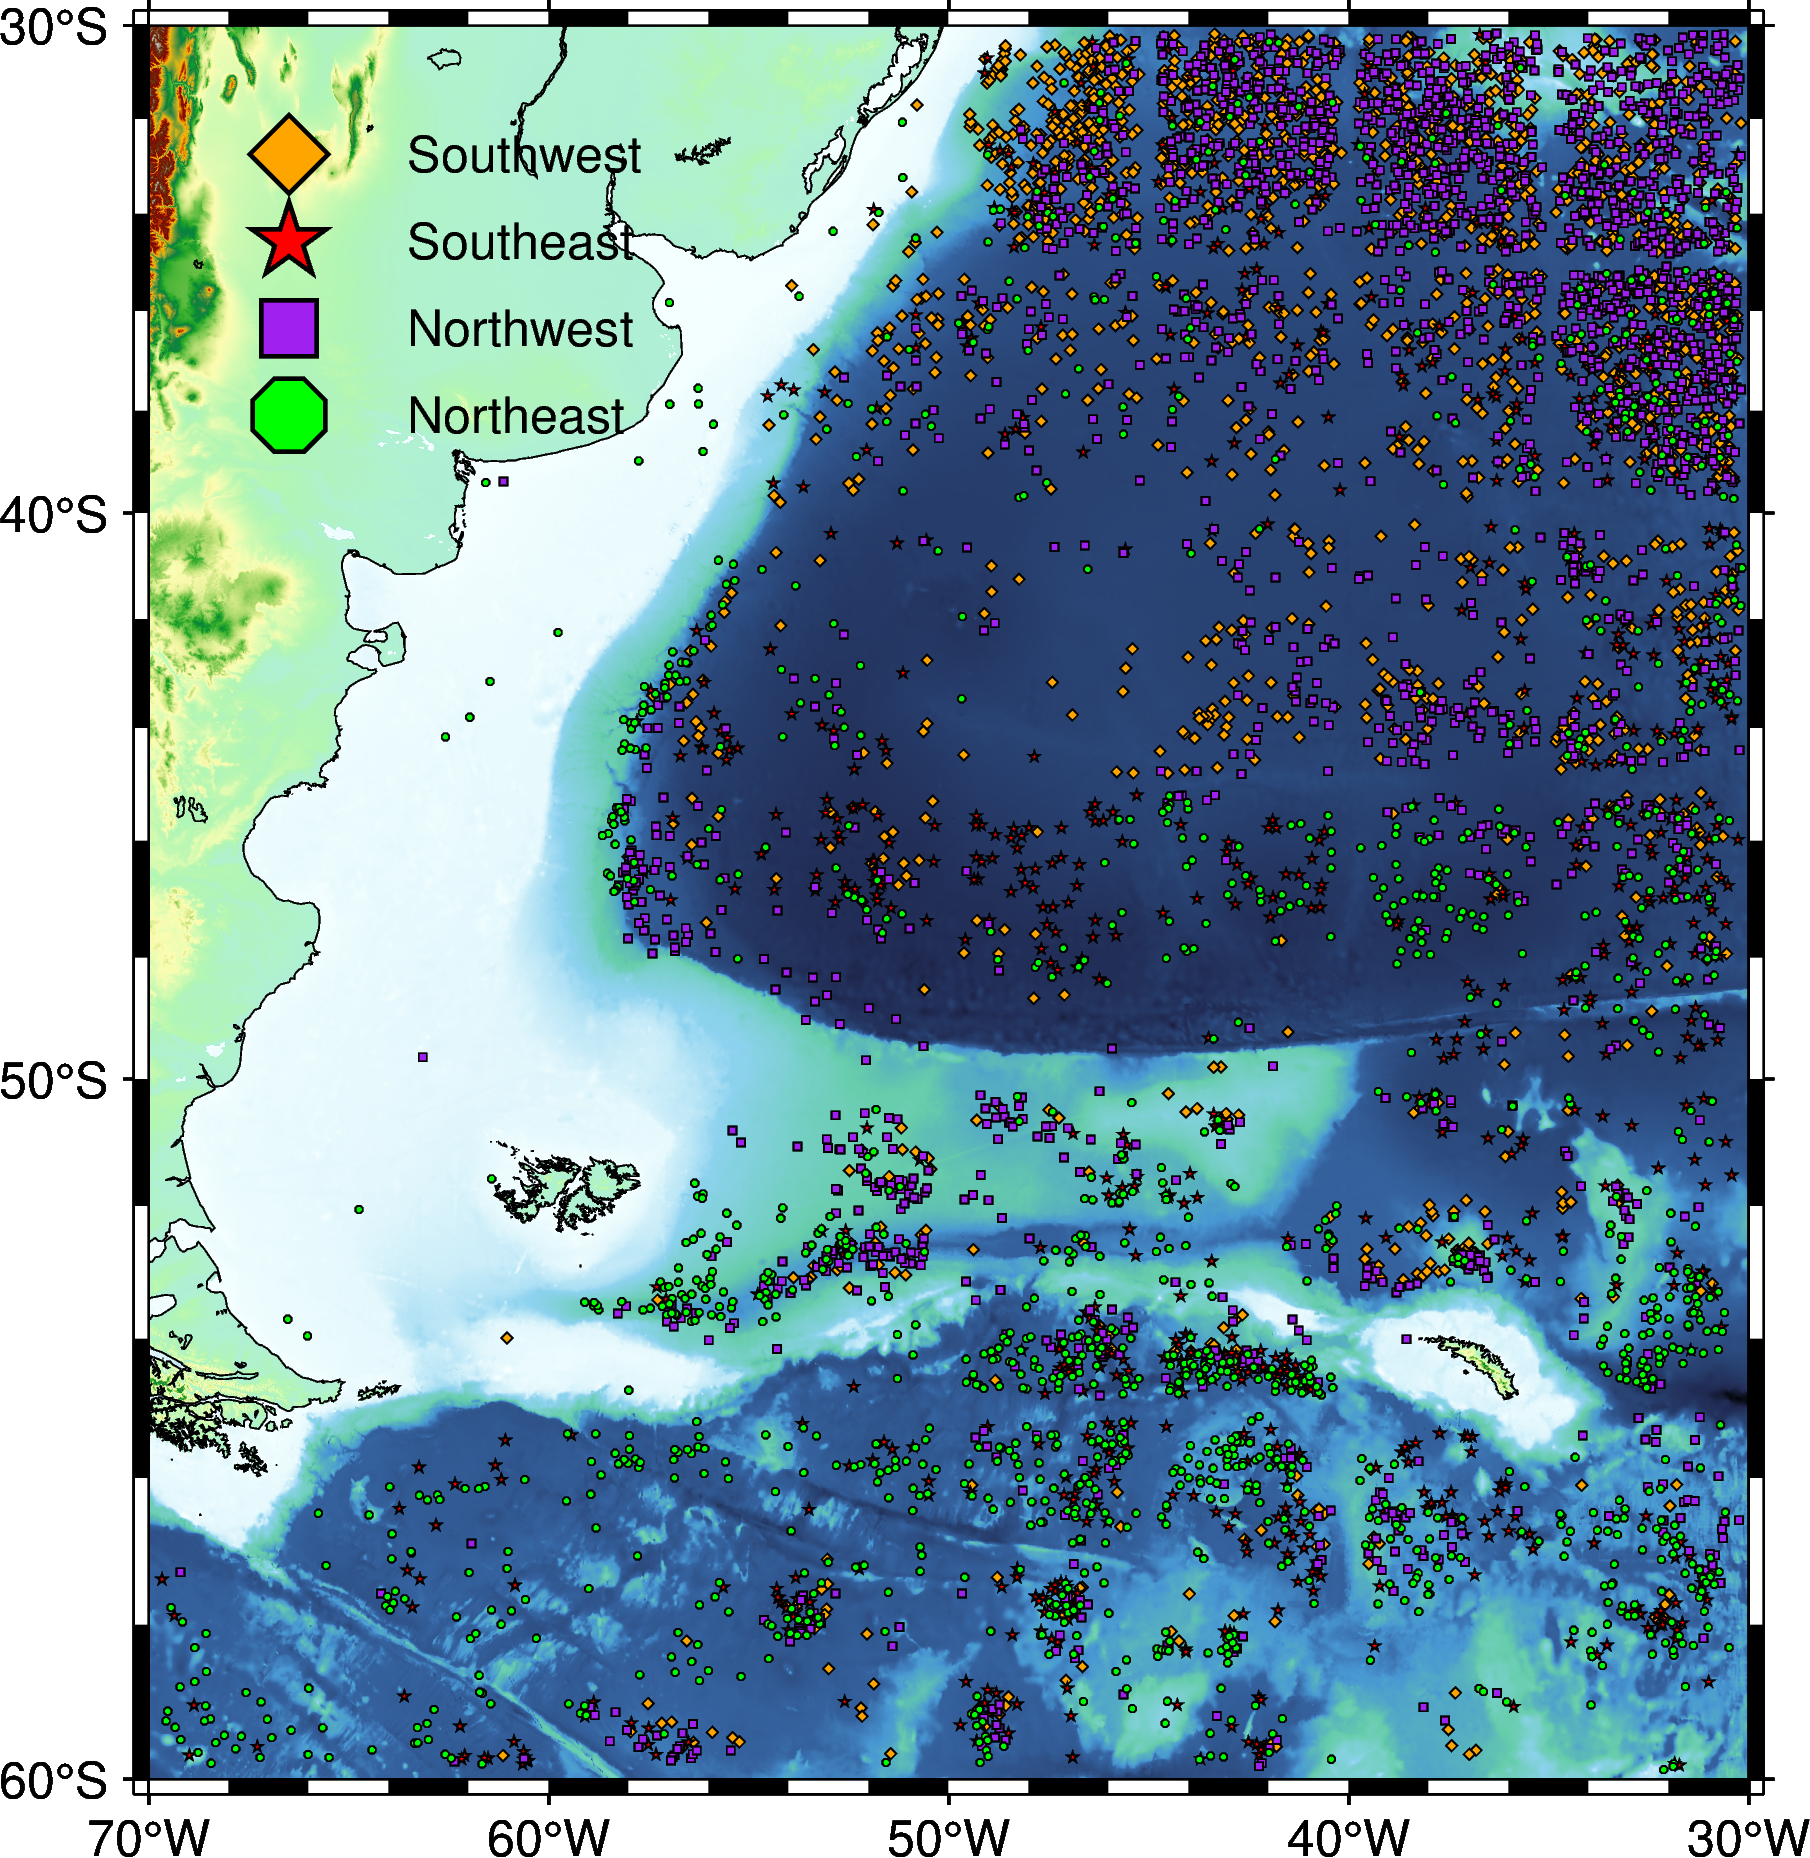
\includegraphics[width = 15cm]{chapter/figure/eddy classification map_SNWE2.png}
    \caption{Eddy travel direction map}
    \label{eddy classification map_SNWE2}
\end{figure}

Figure \ref{some vortex examples} shows some cases study of the  eddies transport path. As shown in section (a) of figure \ref{some vortex examples}, a cyclonic eddy propagates westward in the center of the Argentine Basin. Section b shows an anti-cyclonic eddy on the southern border of the basin and its travel direction is to the southeast. In Section C of the figure, one cyclonic eddy near South Georgia and the South Sandwich Islands goes north and it lost its coherence strongly during the last ten days of transport. Section d of the figure depicts a typical vortex going southward along the South American continental slope, the direction of which is the same as the mean flow thus, a considerable number of vortices are also transported this way.


\begin{figure}
    \centering
    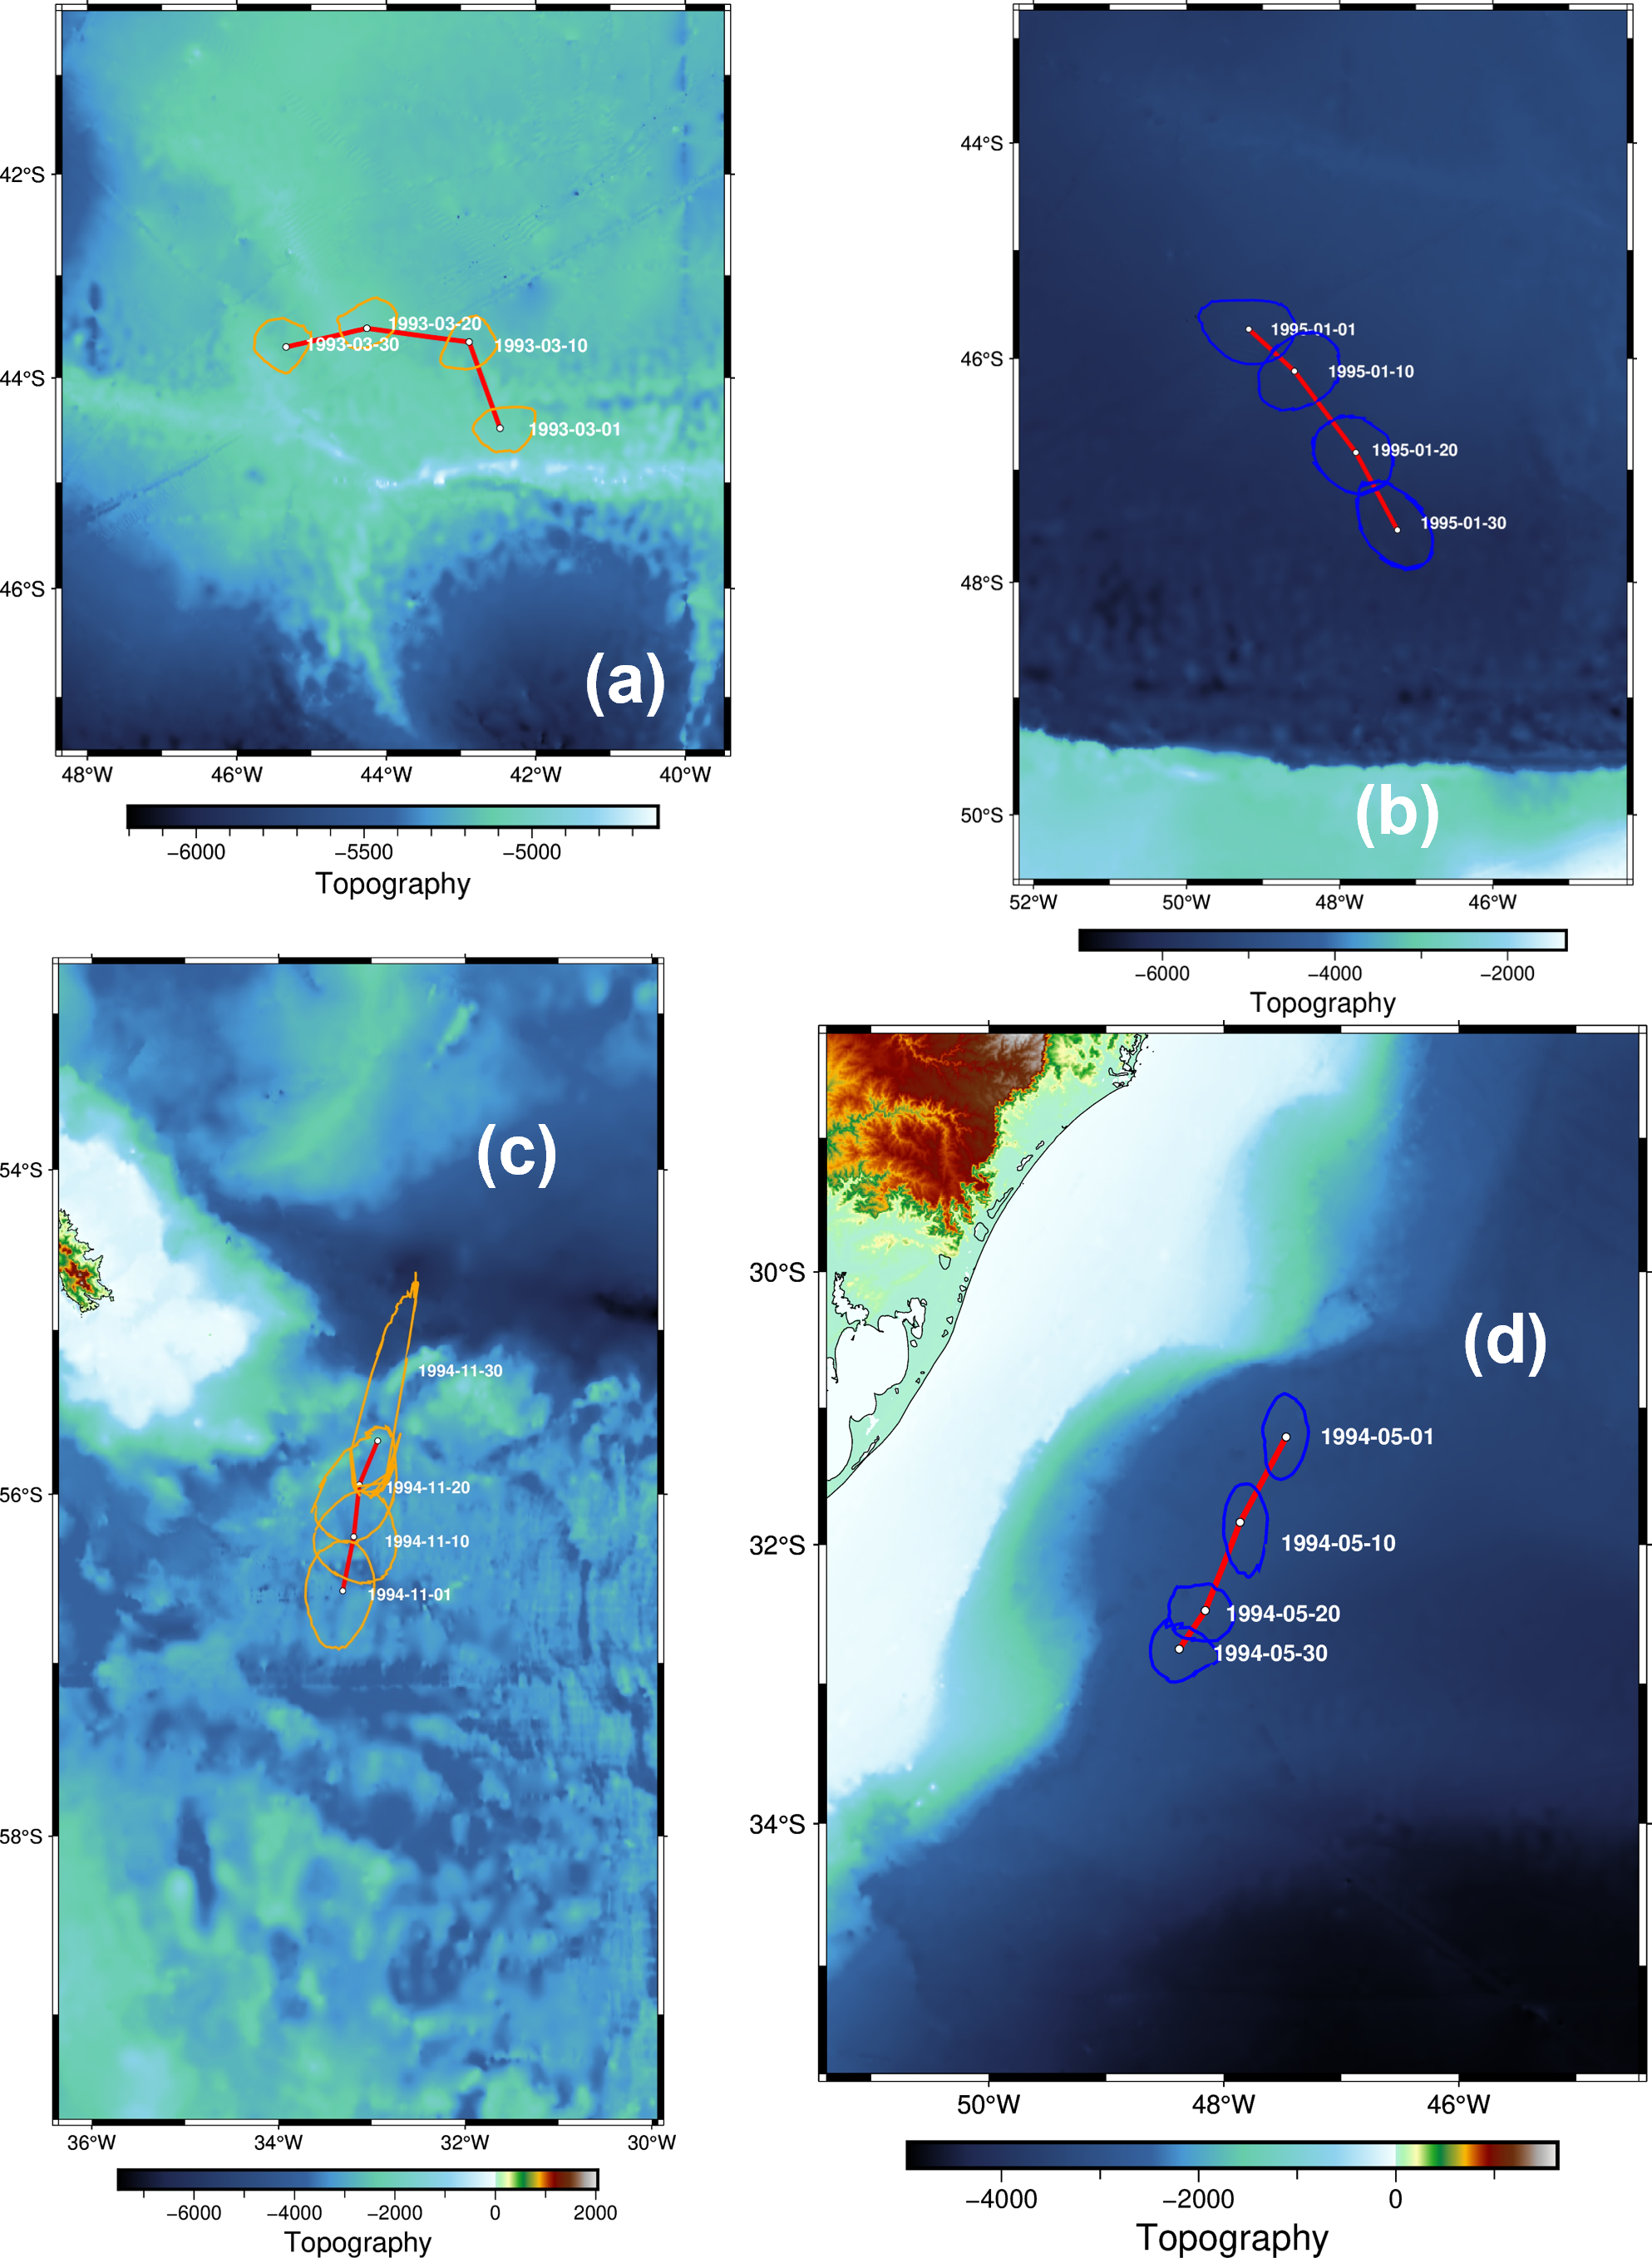
\includegraphics[width = 0.9\textwidth]{chapter/figure/eddy map.png}
    \caption{Some vortex examples (orange for cyclonic eddy and blue for anti-cyclonic eddy)}
    \label{some vortex examples}
\end{figure}

% \section{Eddies morphology}

\section{Eddies coherence time}

In Chapter \ref{Eddies statistics}, we set the coherent time of 30-day and detect 6212 coherent eddies in the study period from 1993 to 2019. However, the properties of the coherent eddy are affected by the selection of time interval to a large extent \cite{xia2022global,vortmeyer2016detecting}.

In the context of the Eulerian detection method (SSHA), the vortex life cycle is defined as the time period of the process of a vortex from birth to death \cite{mccoy2020global,andrade2020genesis}.
According to the previous research, the life cycle of a vortex varies from 4 weeks to  16 weeks and the average life cycle is about 8-9 weeks.

The result is shown in figure \ref{eddy coherent}. From the figure, we could learn that there is a rapid decrease in eddy number when the coherent period is less than 90 days, but the trend slows down after 90 days, which means that an eddy with a life cycle larger than 90 days would tend to survive longer. We could also conclude that eddies with a coherent period of 90 days have the largest radius which suggests that an eddy with a larger radius, magnitude, and intensity will survive longer. 60-day eddies' radius is smaller than 30-day eddies' and 120-day eddies' radius is smaller than 60-day eddies', which 
shows that the time period has an impact on vortex coherence and if we track the eddy exceeding the period $\Delta t$, the outer part of the eddies would be deformed, stretched into filaments, and finally lose coherence.

From figure \ref{eddy type proportion}, we could learn that anticyclonic eddies tend to have larger coherent time. When the coherence period is 30-day, anti-cyclonic eddies only occupy $46\%$ of the total eddy number; while the proportion raise up to $64\%$ when the coherent interval is 120-day.

\begin{figure}[htbp]
    \centering
    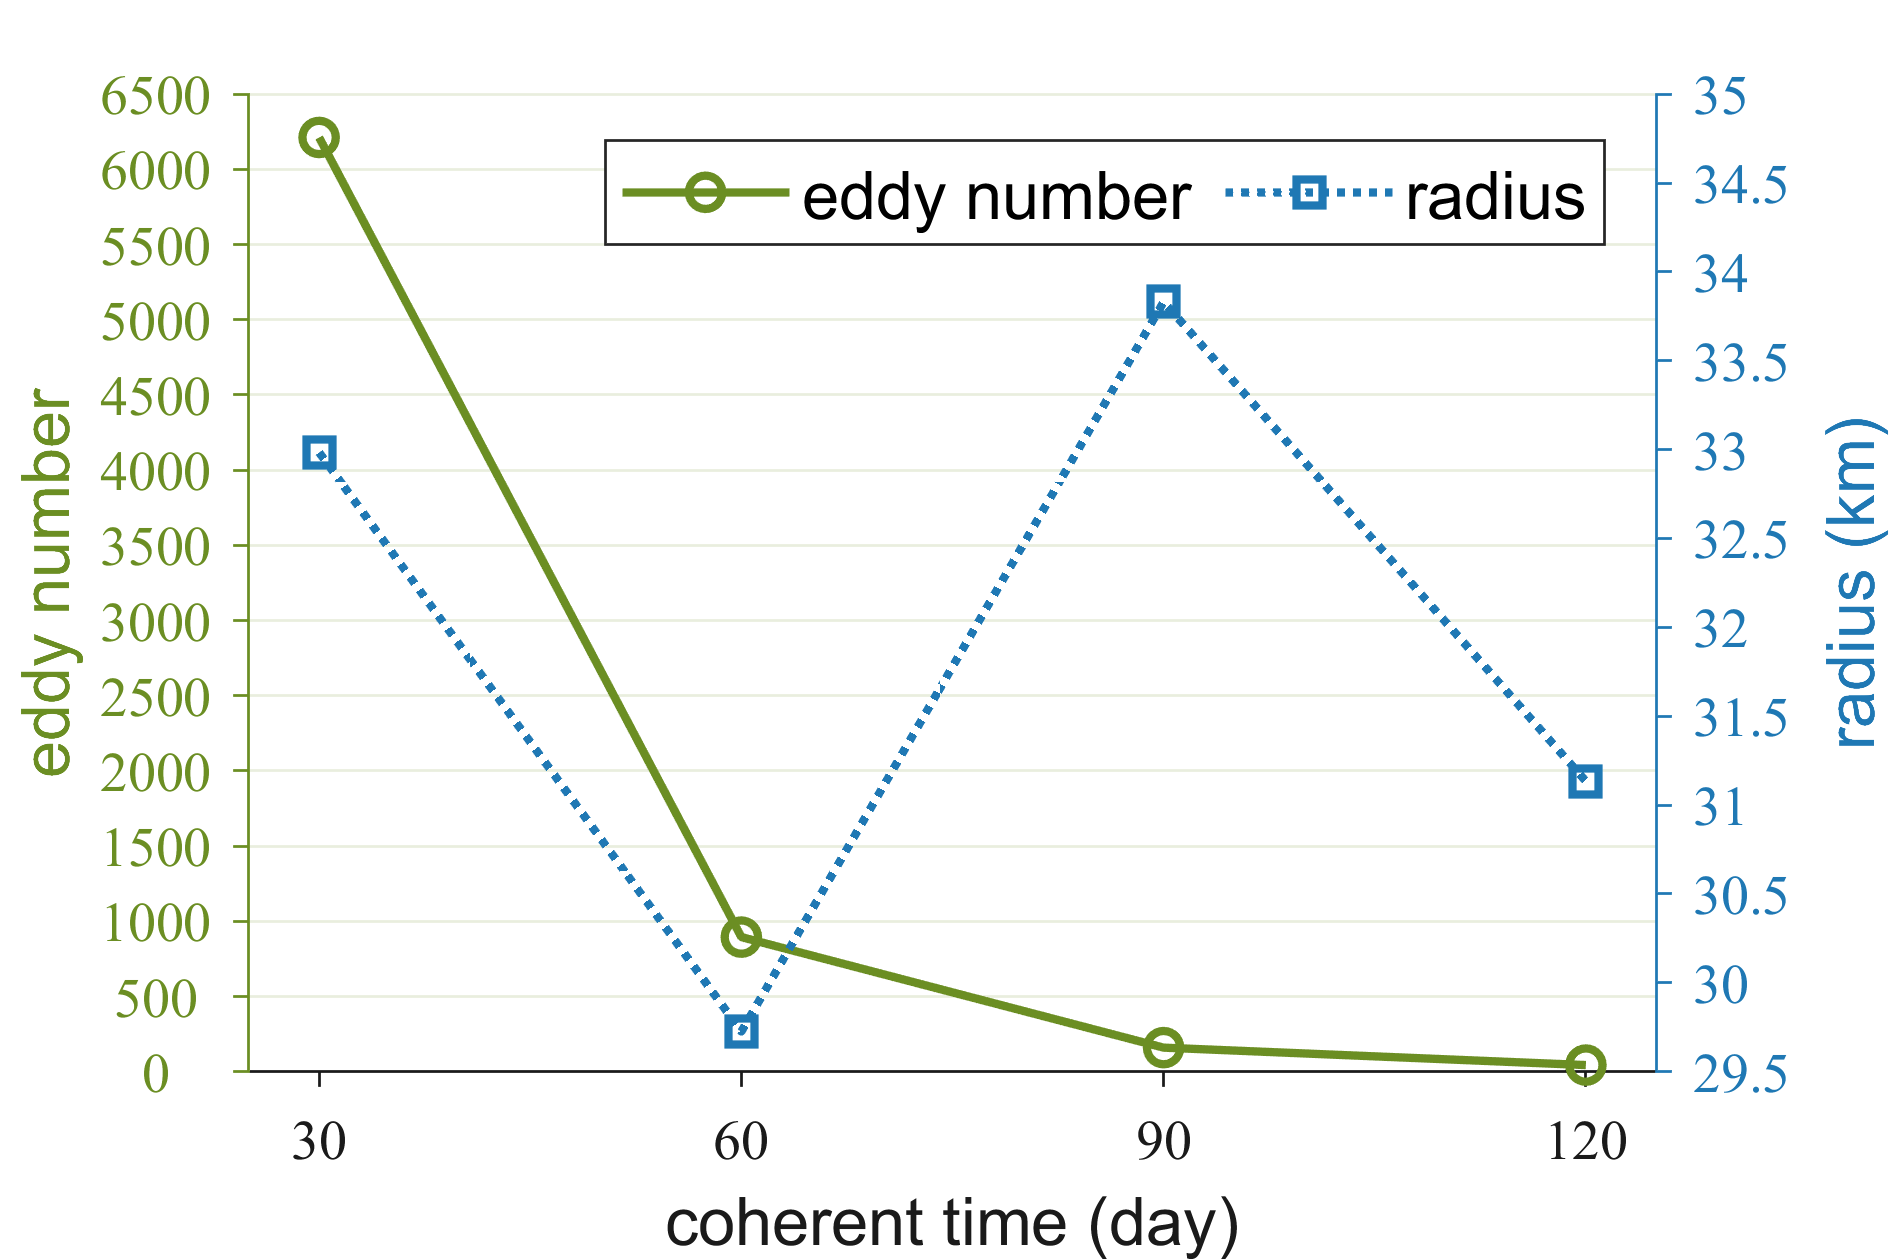
\includegraphics[width = 15cm]{chapter/figure/eddy coherent.png}
    \caption{Eddy properties and their relationship with coherence time}
    \label{eddy coherent}
\end{figure}

\begin{figure}[htbp]
    \centering
    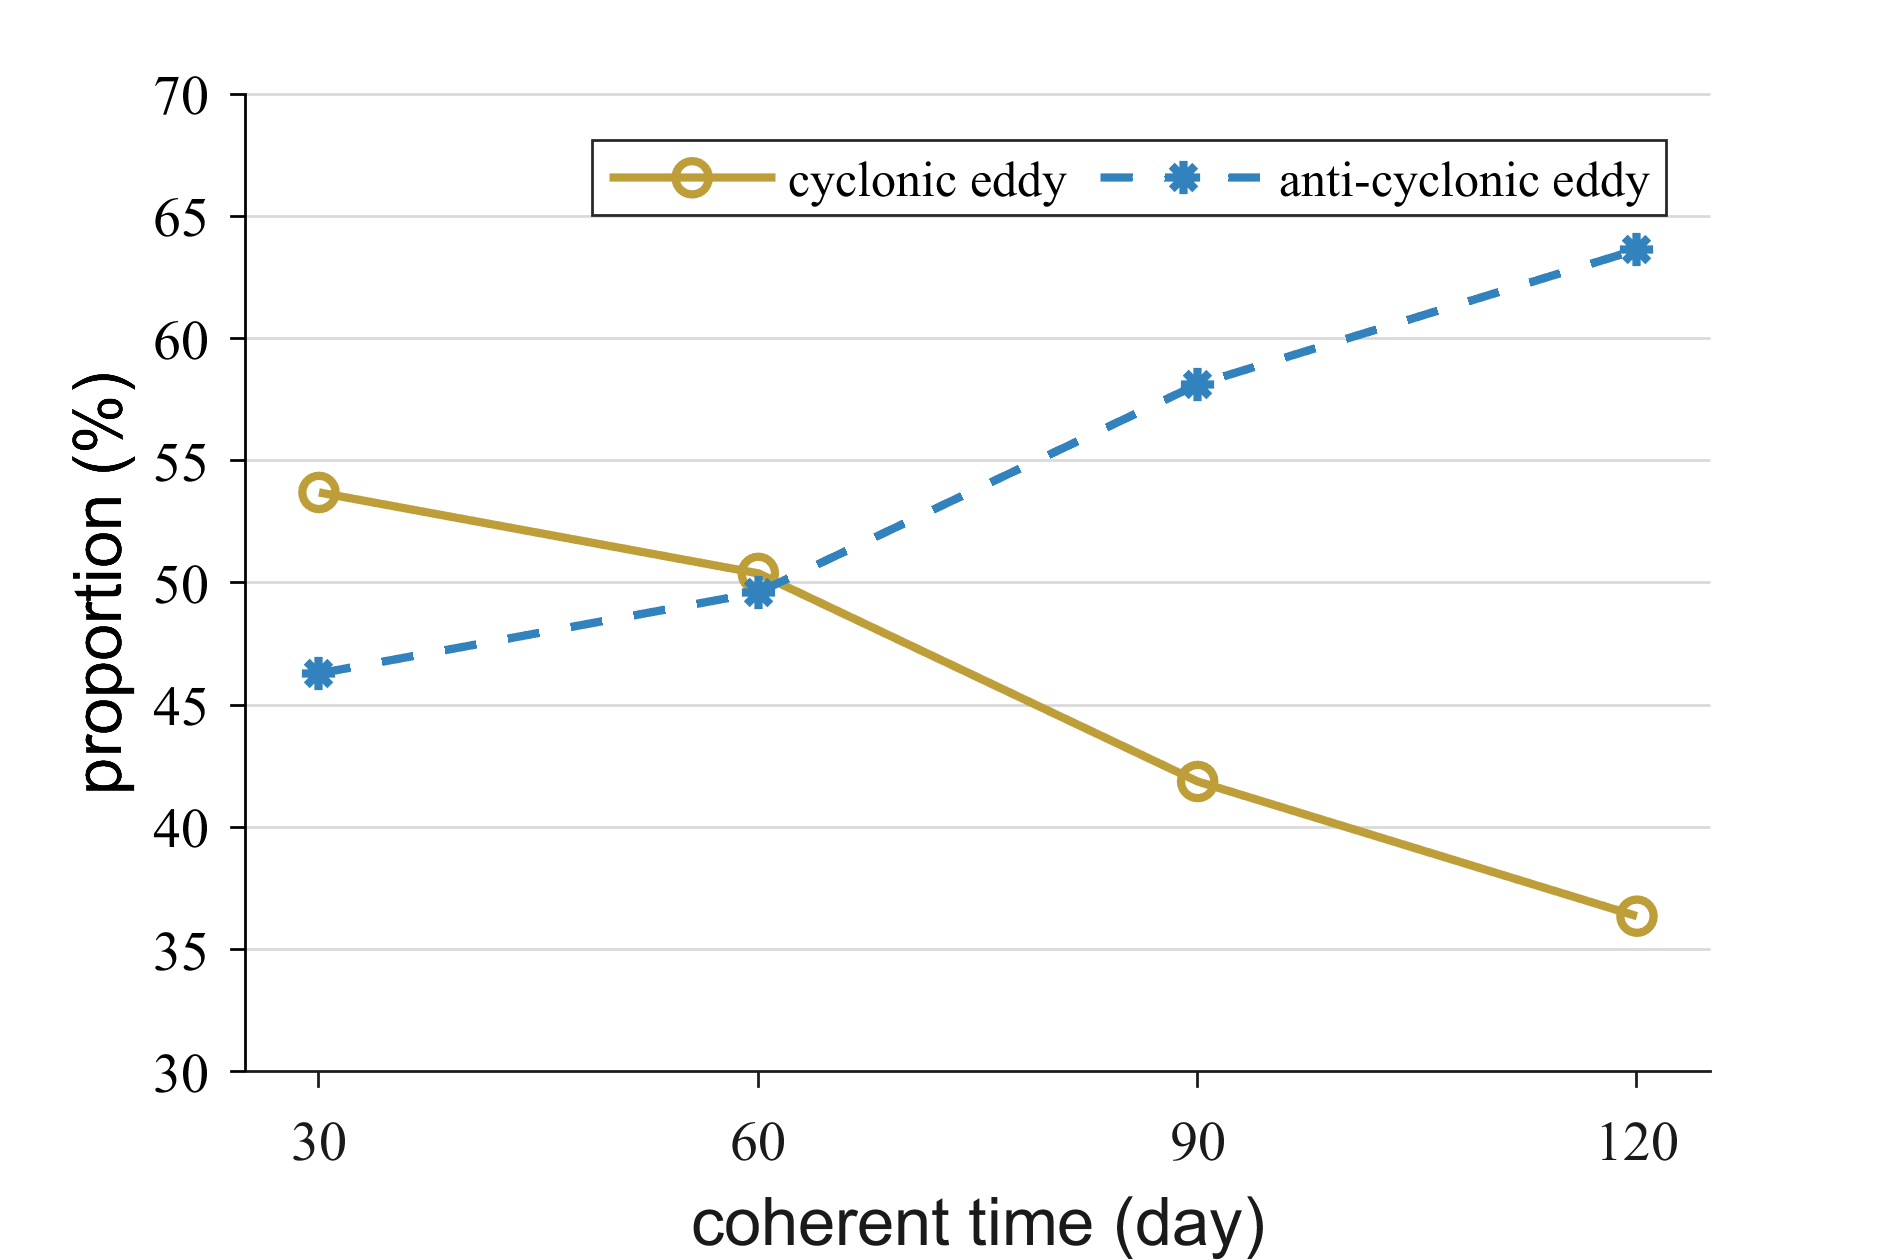
\includegraphics[width = 15cm]{chapter/figure/eddy type proportion.png}
    \caption{Eddy type proportion map}
    \label{eddy type proportion}
\end{figure}

Figure \ref{120-day eddies} shows three detected eddies with a coherent time of 120 days. In section (a) of the figure, the coherent time of the anti-cyclonic eddy originated in January 1998, the anti-cyclonic eddy shown in section (b) of the figure stemmed from September 2006 while the cyclonic eddy in section (c) was calculated using $t_0= September 2019$.In the figure, the initial position is marked with a black circle and the final position is marked in orange; anti-cyclonic eddy is indicated in red while cyclonic eddy is indicated in blue. They all show a westward propagation trend, carry water masses from the east to the west boundary, and finally the sea surface signal piles up at the west. 

\begin{figure}[htbp]
    \centering
    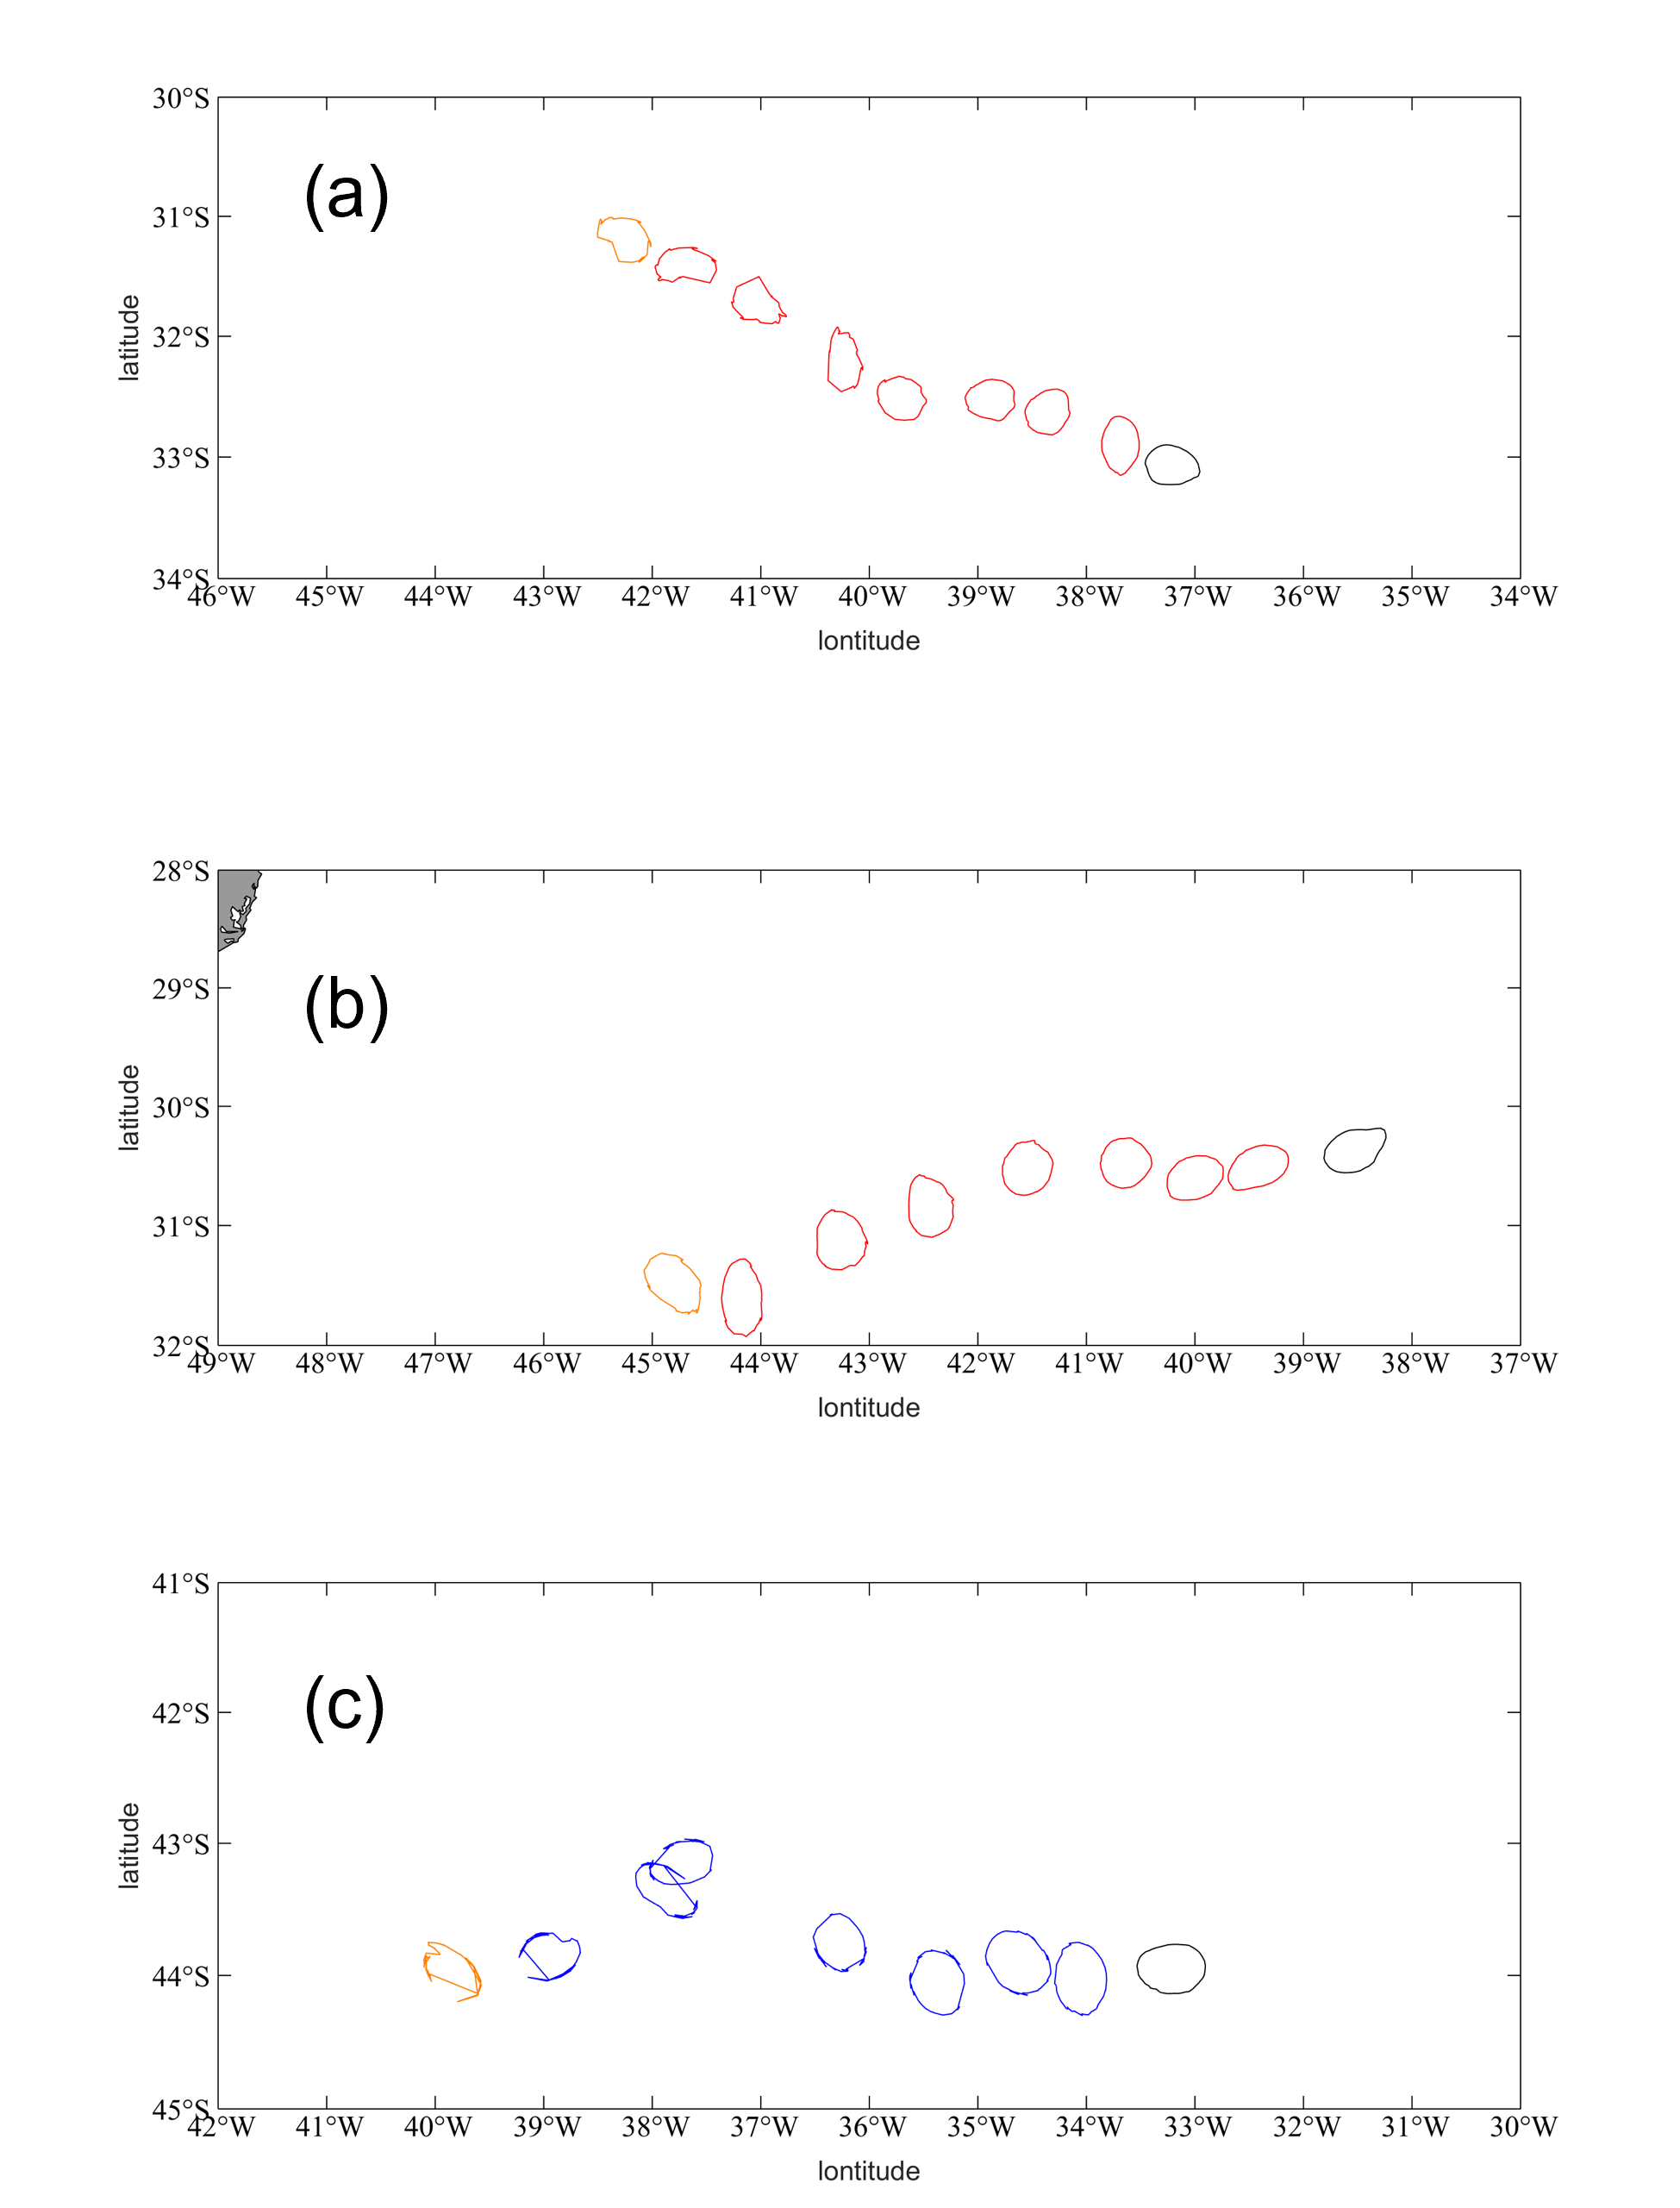
\includegraphics[width = 15cm]{chapter/figure/120-day eddies.png}
    \caption{Trajectories map of three 120-day vortices}
    \label{120-day eddies}
\end{figure}

\newpage

\section{Conclusion}

According to the criterion of the LAVD method, we have detected a total of 6212 coherent vortices, including 3336 cyclonic vortices and 2876 anticyclonic vortices from 1993 to 2019. There is an upward trend of eddies number. From the statistical results, there are obvious seasonal changes in the generation of anticyclonic vortices, which are more in spring and summer and less in autumn and winter.

Analysis of regional eddy statistics reveals hot spots of generation in the northeast part of the Argentine Basin and reveals the limitations of the LAVD method in high latitude regions and coastal shallow waters.

Lots of eddies have been observed in the southwest part of the Argentine Basin where Brazil Malvinas Confluence gives rise to baroclinic instabilities. The Center part of the Argentine Basin is associated with an eddy-free zone. The northern part of the Argentine Basin and connecting region between the Southern Ocean and the Argentine Basin are also the hot-spot of the oceanic eddy.

Eddies' radius decrease when the latitude is higher and the propagation speed is the largest in the middle latitude.

Vortex polarity has an effect on vortex properties: anticyclonic eddies are more stable and tend to have larger coherent time.





